\documentclass{article}

\usepackage[T1]{fontenc}
\usepackage[utf8]{inputenc}
\usepackage[brazilian]{babel}
\usepackage{graphicx}
\usepackage[export]{adjustbox}[2011/08/13]
\usepackage{float}
\usepackage[pdftex]{hyperref}
\usepackage{epstopdf}
\usepackage{etoolbox}
\usepackage{amsmath}
\usepackage{amsfonts}
\usepackage{amssymb}
\usepackage{caption}
\usepackage{subcaption}
\usepackage{setspace}
\usepackage{tikz}
\usepackage{listings}
\usepackage{xcolor} 

\bibliographystyle{eric}
\patchcmd{\thebibliography}{\section*}{\section}{}{}


\newcommand{\R}{\ensuremath{\mathbb{R}}}
\newcommand{\Prob}{\ensuremath{\mathbb{P}}}
\newcommand{\K}{\ensuremath{\mathbb{K}}}
\newcommand{\U}{\ensuremath{\mathbb{U}}}
\newcommand{\N}{\ensuremath{\mathbb{N}}}
\newcommand{\Lg}{\ensuremath{\mathbb{L}}}
\newcommand{\T}{\ensuremath{\rm Tr}}
\newcommand{\sg}{{\sigma(x_k)}}

\newcommand{\G}{\ensuremath{\mathcal{G}}}
\newcommand{\F}{\ensuremath{\mathcal{F}}}
\newcommand{\C}{\ensuremath{\mathcal{C}}}
\newcommand{\E}{\ensuremath{\mathcal{E}}}
\newcommand{\Hn}{\ensuremath{\mathcal{H}}}
\newcommand{\Hoo}{\ensuremath{\mathcal{H}_\infty}}
\newcommand{\Hop}{\ensuremath{\mathcal{H}_{op}}}
% --------------------------------------------------
\newtheorem{theo}{Teorema}
\newtheorem{exa}{Exemplo}
\newtheorem{lemm}{Lema}
\newtheorem{coro}{Corolário}
\newtheorem{defn}{Definição}[section]

\begin{document}

\begin{titlepage}
\begin{center}

\newcommand{\HRule}{\rule{\linewidth}{0.5mm}}
% Upper part of the page. The '~' is needed because \\
% only works if a paragraph has started.

\includegraphics[width=0.15\textwidth]{logoUnicamp}~\\[1cm]

\textsc{\LARGE Universidade Estadual de Campinas}\\[1.5cm]

\textsc{\Large Faculdade de Engenharia Mecânica}\\[0.5cm]

% Title
\HRule \\[0.4cm]
{ \huge \bfseries ES664 - Laboratório de Eletrônica para Automação Industrial\\ \vspace{1cm} Relatório - Experimento 4\\
\Large{Acionamento de motor DC} \\[0.4cm] }

\HRule \\[1.5cm]

% Author and supervisor
\begin{minipage}{0.6\textwidth}
\begin{flushleft} \large
\emph{Nome:}\\
Daniel Dello Russo Oliveira\\Marcelli Tiemi Kian
\end{flushleft}
\end{minipage}
\begin{minipage}{0.2\textwidth}
\begin{flushright} \large
\emph{RA}\\ 101918\\117892
\end{flushright}
\end{minipage}

\vfill

% Bottom of the page
{\large \today}

\end{center}
\end{titlepage}


\onehalfspacing
\section{Objetivos}
	Essa simulação tem como objetivo o estudo dos conversores step-down (buck), step-up (boost) e seus modos de condução contínua e descontínua.
	 
\section{Conversor Buck}
Através do Simulink implementamos o conversor step-down detalhado na figura \ref{fig:bsim}.
\begin{figure}[H]
	\centering
	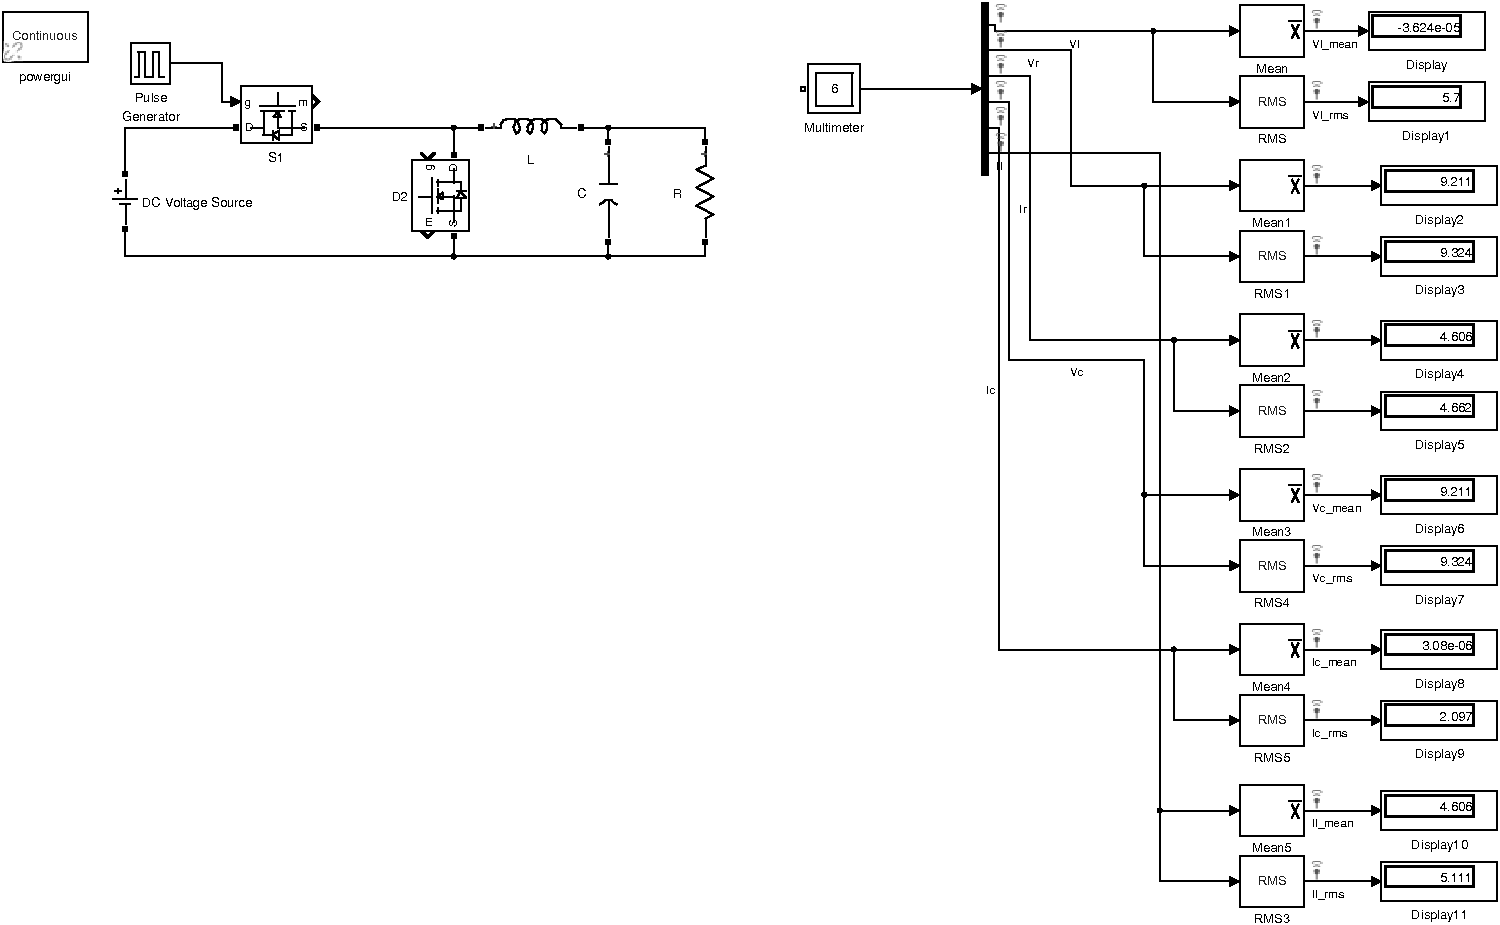
\includegraphics[width=\linewidth]{matlab/buck/bsim}
	\caption{Esquema para simulação do conversor buck}
	\label{fig:bsim}
\end{figure}
Conforme detalhados no roteiro, setamos os parâmetros $R$ = $2\Omega$, $C$ = $220\mu F$, $L$ = $330\mu H$ e simulamos o sistema com uma frequência $f$ = $1kHz$ e duty-cicle de 80\% na chave S1.
Extraímos dessa simulação as curvas de tensão e corrente na carga (figura \ref{fig:br}), no indutor (figura \ref{fig:bl}), no capacitor (figura \ref{fig:bc}), na chave S1 (figura \ref{fig:bs1}) e no diodo D2 (figura \ref{fig:bd2}).
\begin{figure}[H]
	\centering
	\begin{subfigure}[b]{0.4\linewidth}
		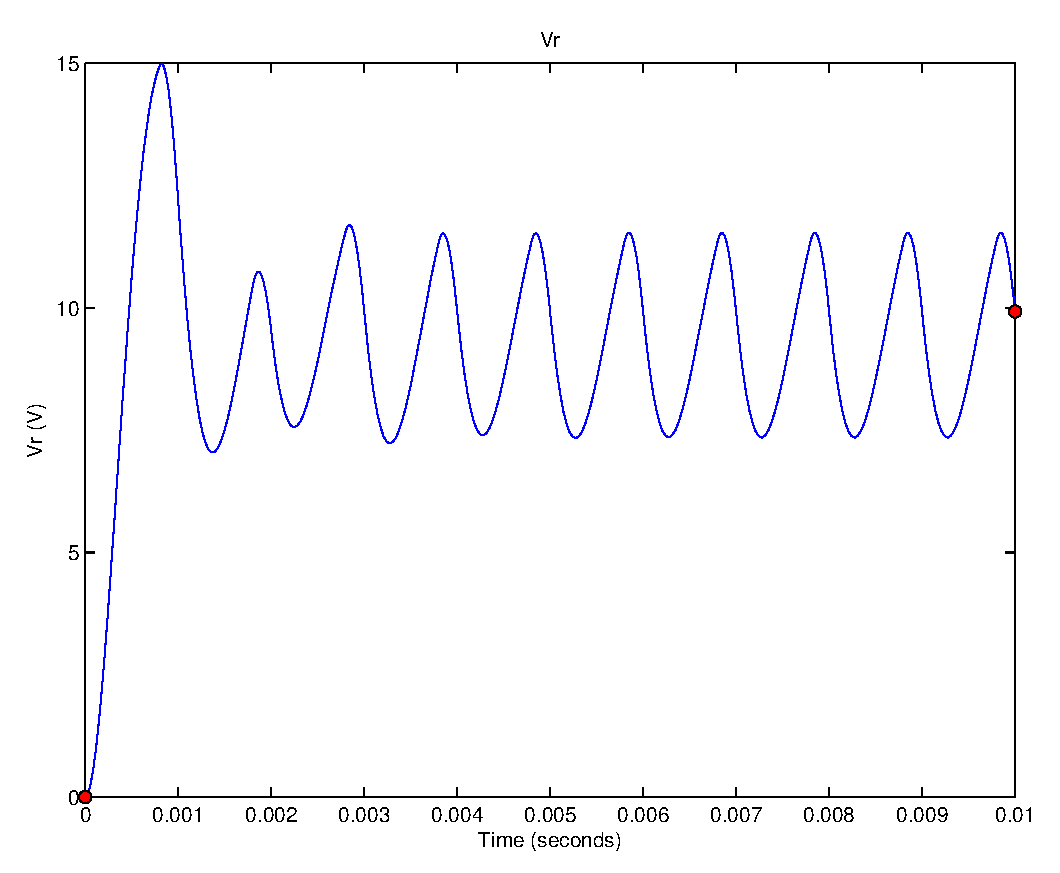
\includegraphics[width=\linewidth]{matlab/buck/b_vr}
		\caption{Tensão no resistor}
	\end{subfigure}
	\begin{subfigure}[b]{0.4\linewidth}
		\centering
		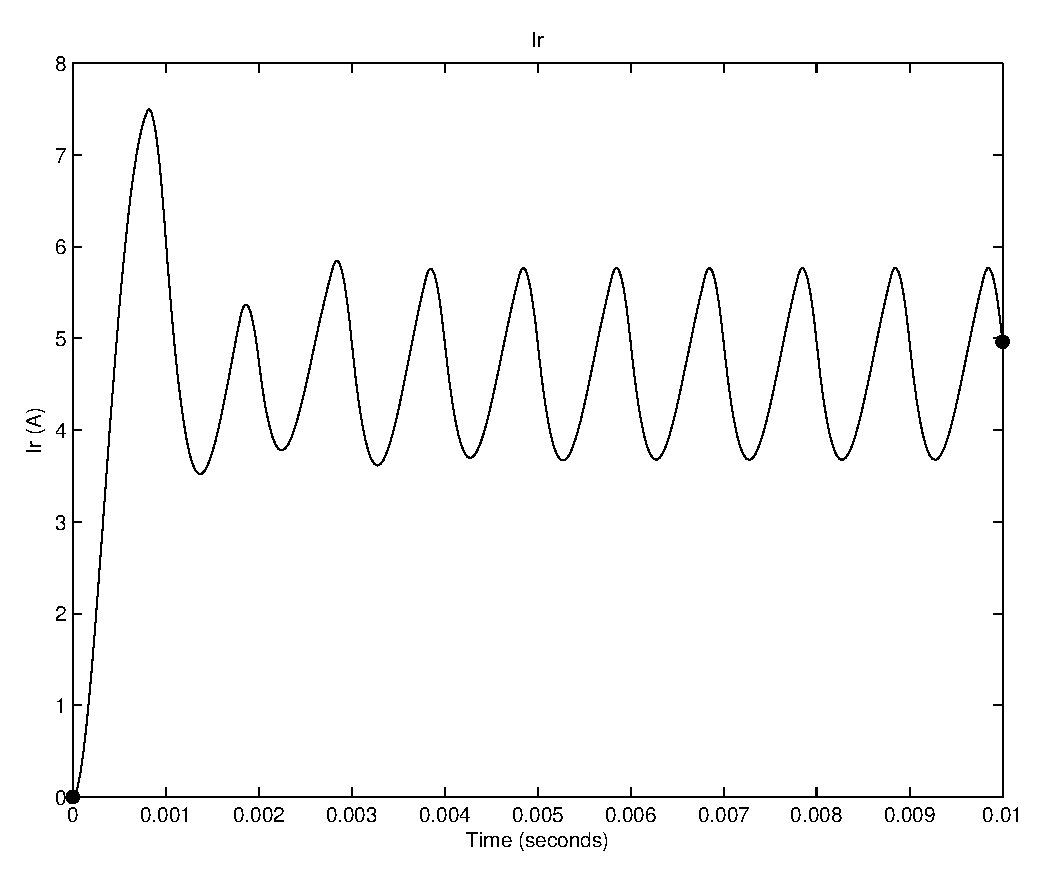
\includegraphics[width=\linewidth]{matlab/buck/b_ir}
		\caption{Corrente no resistor}
	\end{subfigure}
	\caption{Curvas do resistor para conversor buck}
	\label{fig:br}
\end{figure}
\begin{figure}[H]
	\centering
	\begin{subfigure}[b]{0.4\linewidth}
		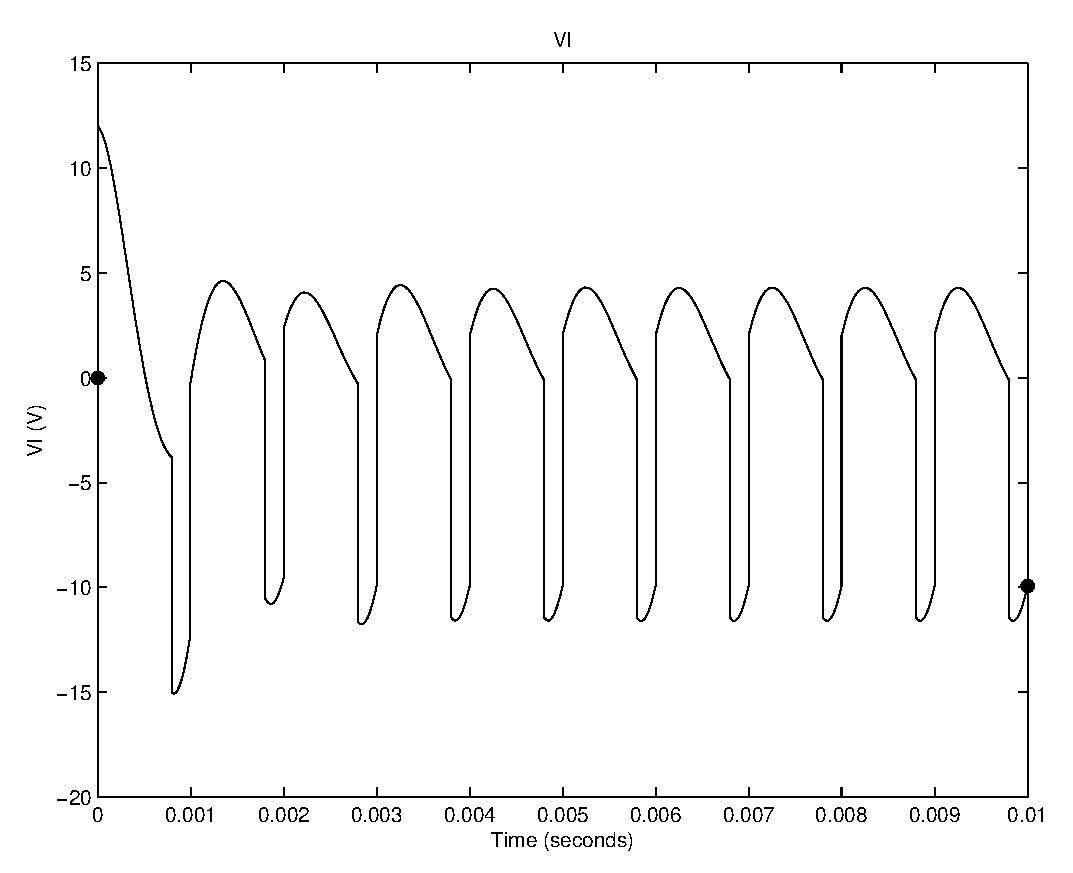
\includegraphics[width=\linewidth]{matlab/buck/b_vl}
		\caption{Tensão no indutor}
	\end{subfigure}
	\begin{subfigure}[b]{0.4\linewidth}
		\centering
		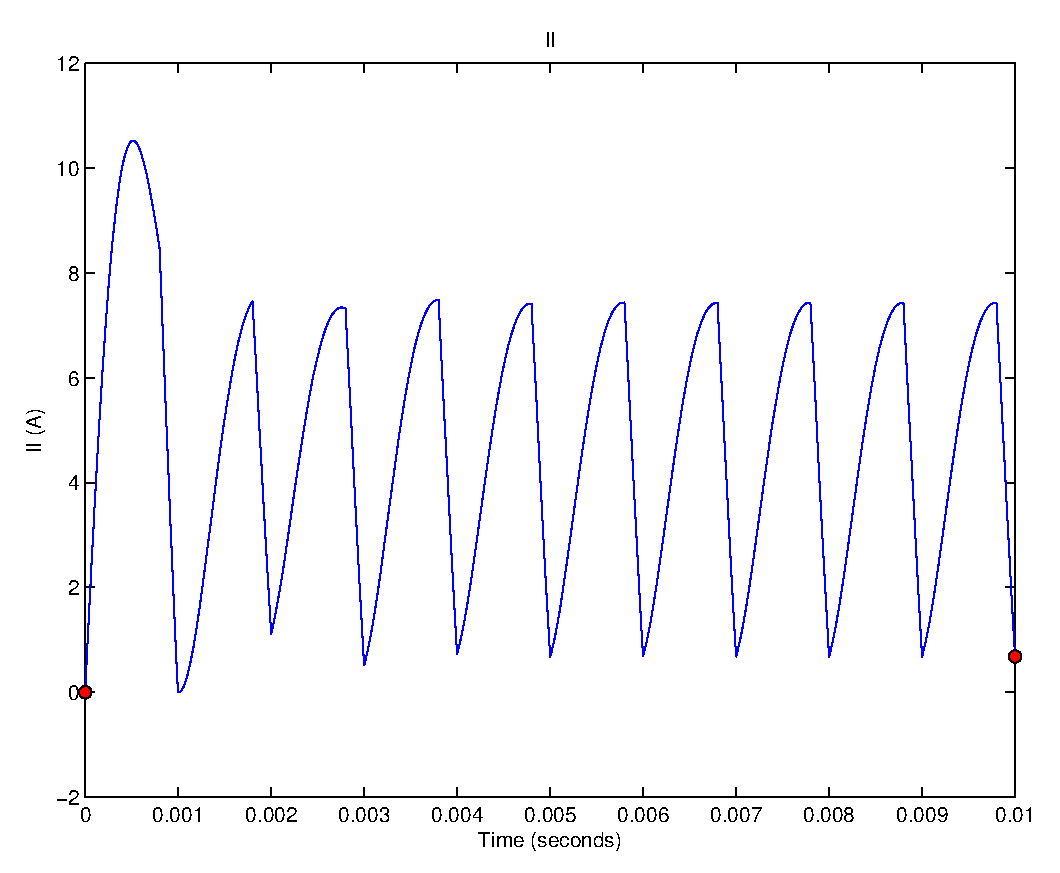
\includegraphics[width=\linewidth]{matlab/buck/b_il}
		\caption{Corrente no indutor}
	\end{subfigure}
	\caption{Curvas do indutor para conversor buck}
	\label{fig:bl}
\end{figure}
\begin{figure}[H]
	\centering
	\begin{subfigure}[b]{0.4\linewidth}
		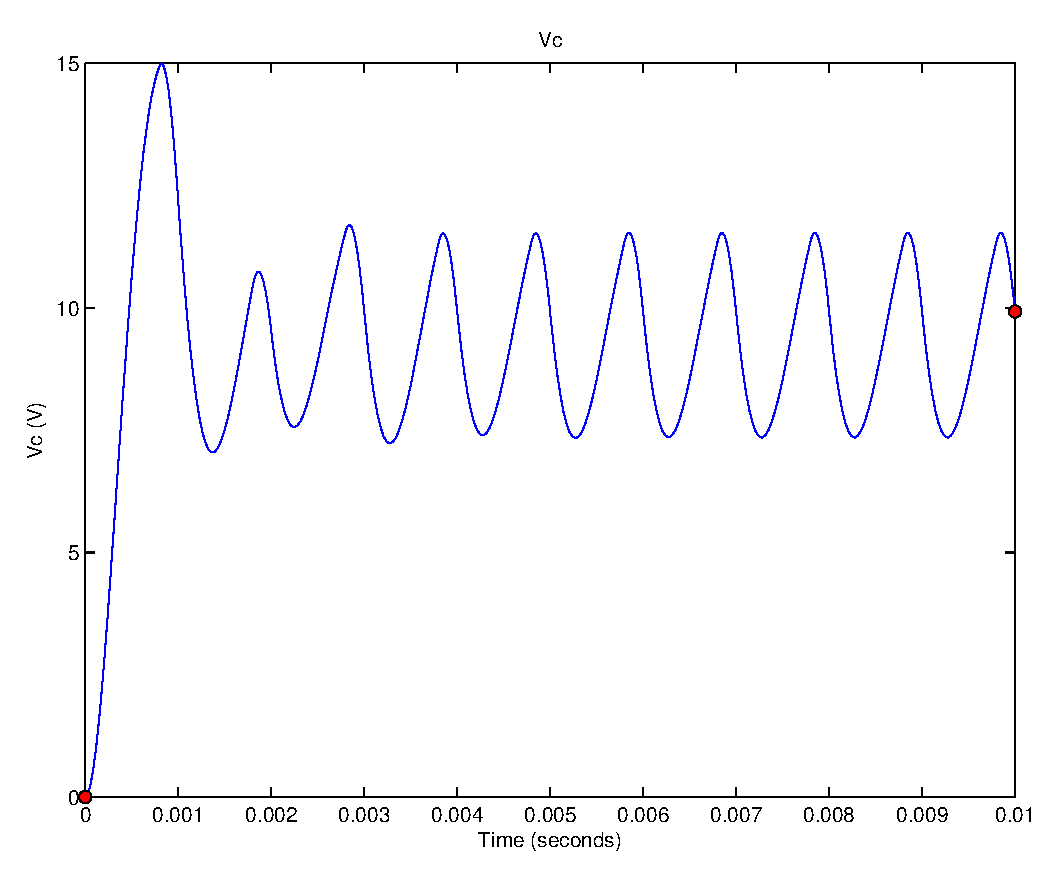
\includegraphics[width=\linewidth]{matlab/buck/b_vc}
		\caption{Tensão no capacitor}
	\end{subfigure}
	\begin{subfigure}[b]{0.4\linewidth}
		\centering
		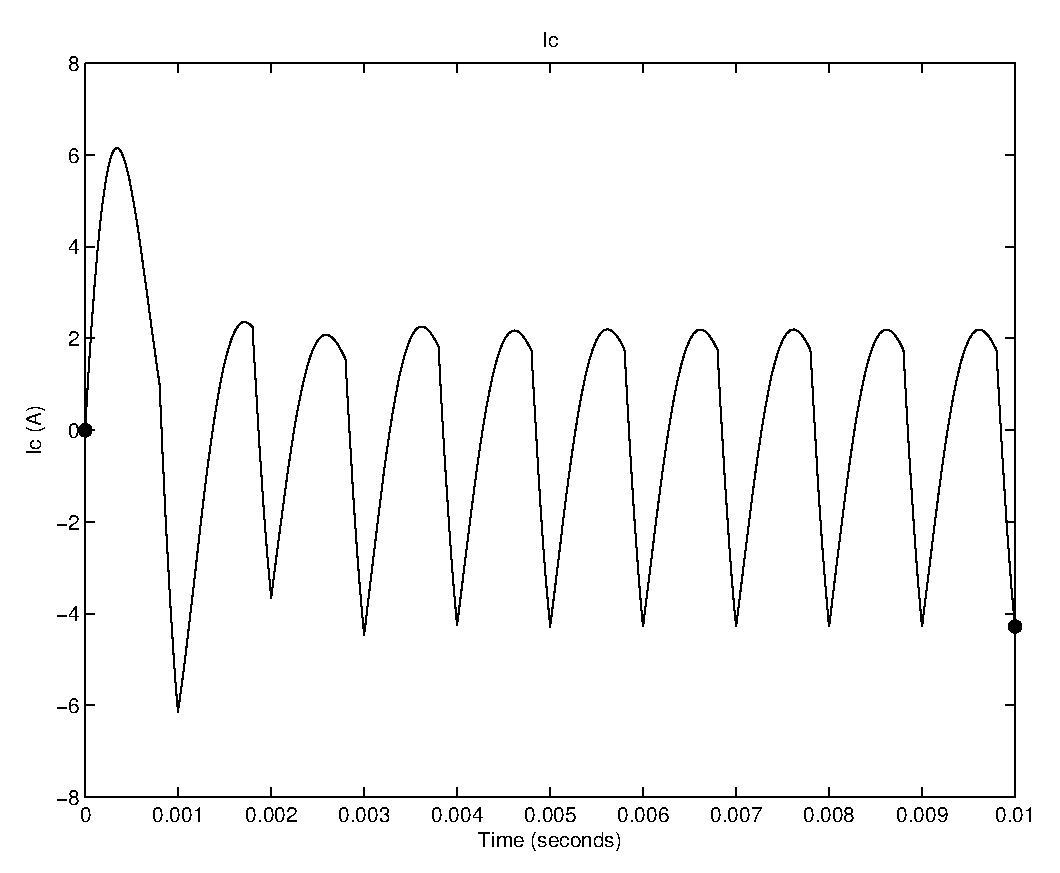
\includegraphics[width=\linewidth]{matlab/buck/b_ic}
		\caption{Corrente no capacitor}
	\end{subfigure}
	\caption{Curvas do capacitor para conversor buck}
	\label{fig:bc}
\end{figure}
\begin{figure}[H]
	\centering
	\begin{subfigure}[b]{0.4\linewidth}
		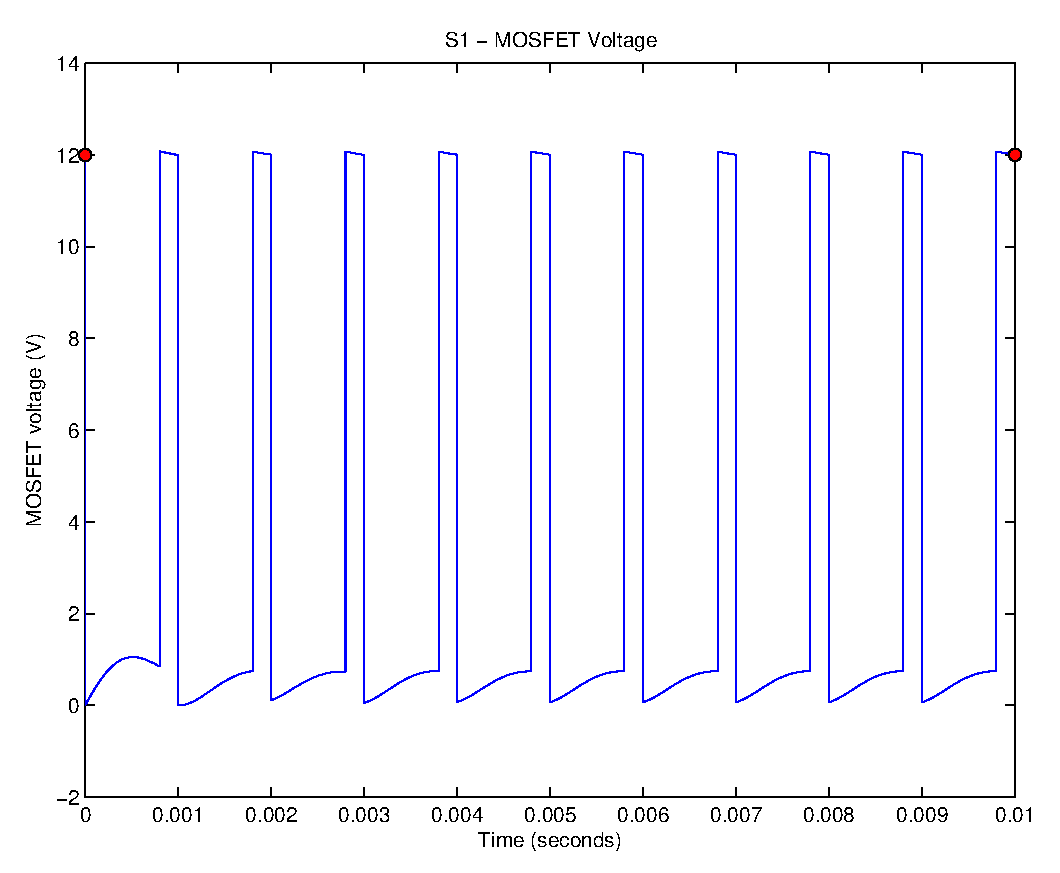
\includegraphics[width=\linewidth]{matlab/buck/r_s1v}
		\caption{Tensão na chave S1}
	\end{subfigure}
	\begin{subfigure}[b]{0.4\linewidth}
		\centering
		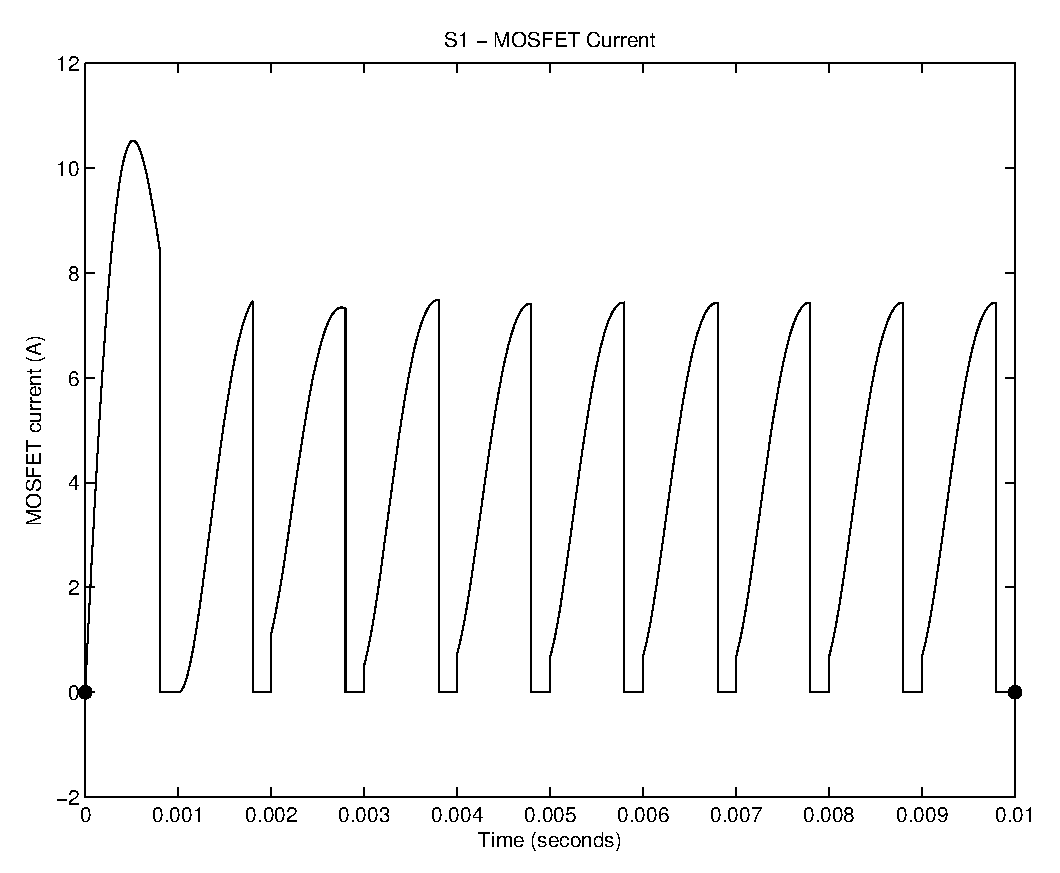
\includegraphics[width=\linewidth]{matlab/buck/r_s1i}
		\caption{Corrente na chave S1}
	\end{subfigure}
	\caption{Curvas da chave S1 para conversor buck}
	\label{fig:bs1}
\end{figure}
\begin{figure}[H]
	\centering
	\begin{subfigure}[b]{0.4\linewidth}
		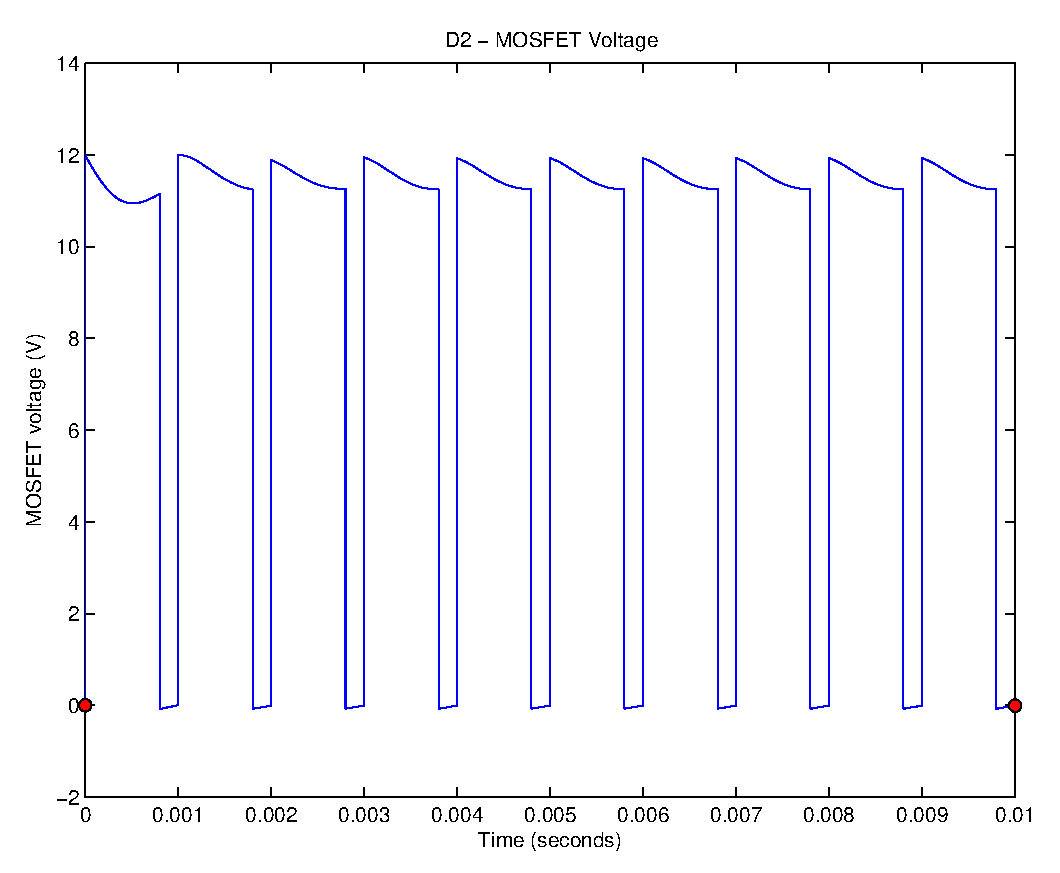
\includegraphics[width=\linewidth]{matlab/buck/r_d2v}
		\caption{Tensão no diodo D2}
	\end{subfigure}
	\begin{subfigure}[b]{0.4\linewidth}
		\centering
		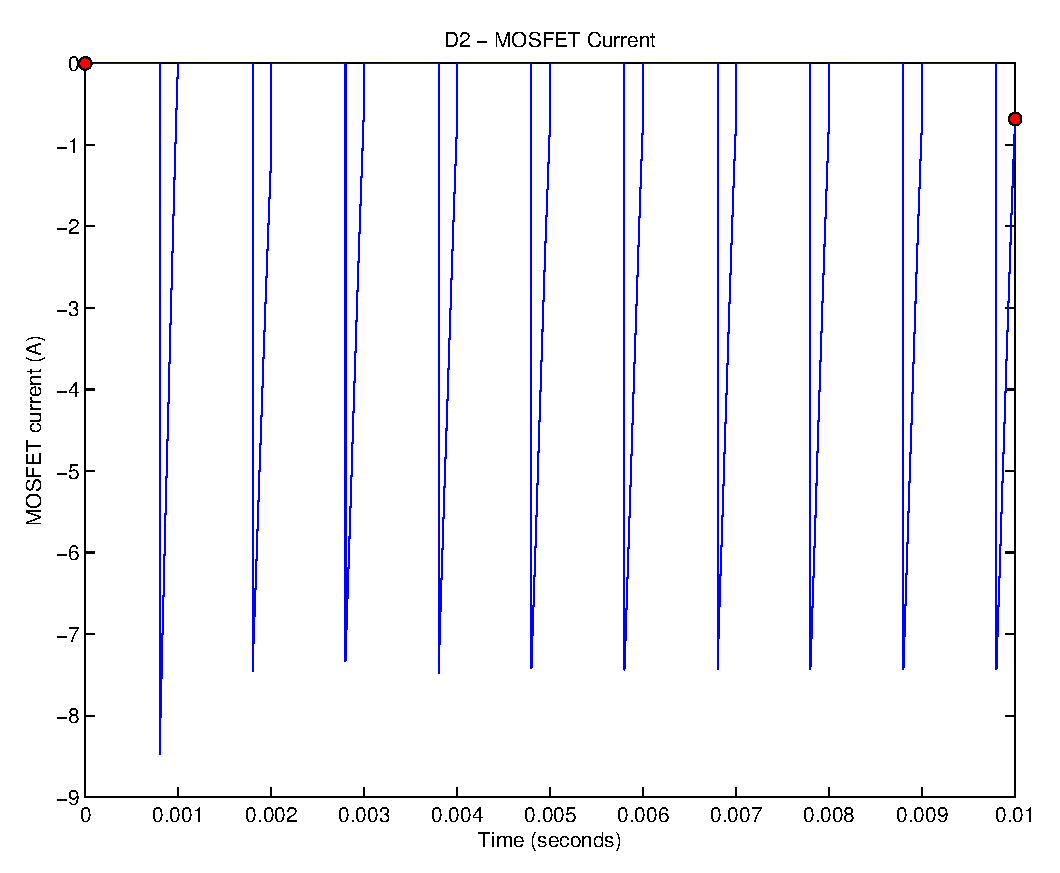
\includegraphics[width=\linewidth]{matlab/buck/r_d2i}
		\caption{Corrente no diodo D2}
	\end{subfigure}
	\caption{Curvas do diodo D2 para conversor buck}
	\label{fig:bd2}
\end{figure}

Medimos as tensões média e efetiva no resistor, obtendo os seguintes valores:
\begin{equation}
\overline{Vr} = 9.2111\ V
\end{equation}
\begin{equation}
Vr_{rms} = 9.3240\ V
\end{equation}

Conforme podemos ver analisando as curvas, %TODO

Podemos calcular a tensão média teórica sobre a carga através da equação \ref{eq:bumean}
%TODO
\begin{equation}
\overline{Vr} = 
\label{eq:bumean}
\end{equation}

Variamos então o valor do duty-cicle entre 0 e 100\% e encontramos a tensão média sobre a carga. Comparamos esse valor com o valor teórico esperado na figura \ref{fig:buvrxd}
\begin{figure}[H]
	\centering
	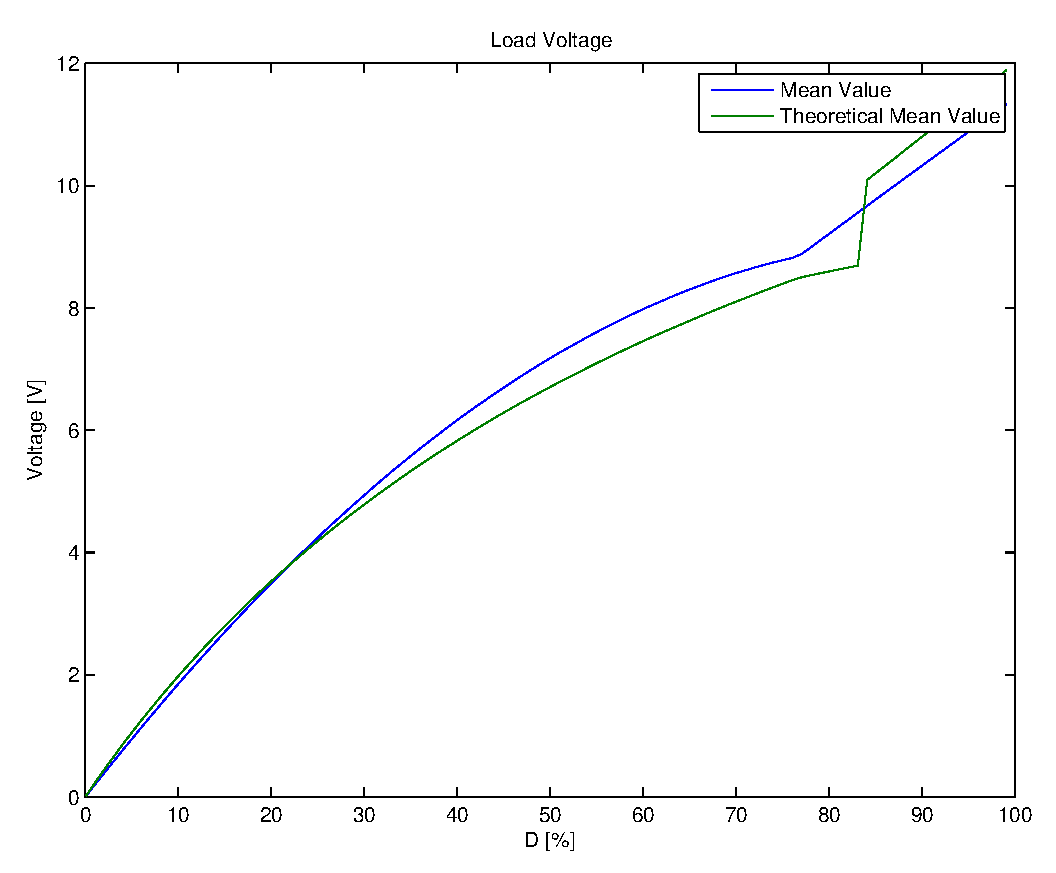
\includegraphics[width=0.7\linewidth]{matlab/buck/r_vrxd}
	\caption{Tensão média no resistor para conversor buck}
	\label{fig:buvrxd}
\end{figure}

Como podemos ver os valores obtidos são %TODO esperados teoricamente, isso se deve às imprecisões numéricas da simulação, à queda de tensão introduzida pelos diodos, ao pequeno período de amostragem, entre outros fatores.

Podemos calcular o valor da indutância limite $L_b$ para que o conversor trabalhe em modo de condução contínua utilizando a equação:
\begin{equation}
	L_b = \frac{(1 - D)R}{2f_s}
\end{equation}
Para um duty-cicle $D$ = $80\%$, temos:
\begin{equation}
	L_b = 400\mu H
\end{equation}

Ajustamos então nosso indutor para $L$ = $\frac{L_b}{2}$ = $200 \mu H$ e rodamos a simulação novamente, obtendo os resultados apresentados nas figuras \ref{fig:br2}, \ref{fig:bl2}, \ref{fig:bc2}, \ref{fig:bs12}, \ref{fig:bd22}.

\begin{figure}[H]
	\centering
	\begin{subfigure}[b]{0.4\linewidth}
		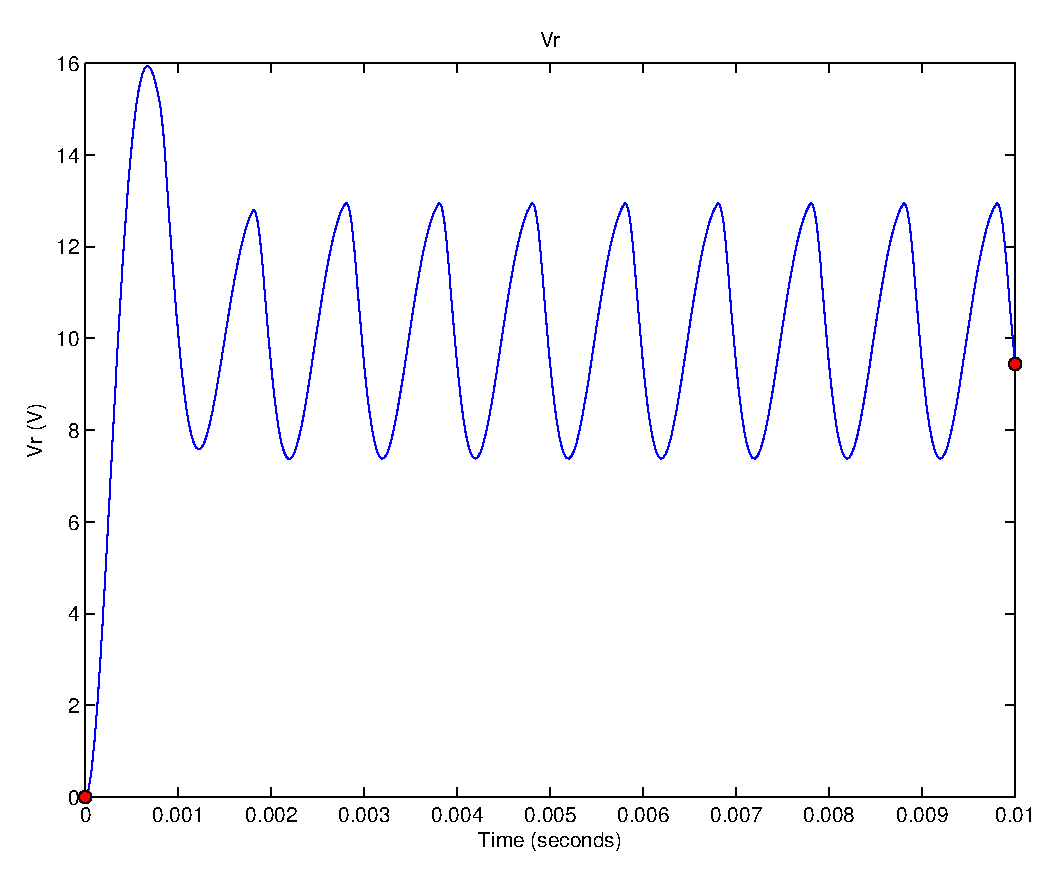
\includegraphics[width=\linewidth]{matlab/buck/b_vr2}
		\caption{Tensão no resistor}
	\end{subfigure}
	\begin{subfigure}[b]{0.4\linewidth}
		\centering
		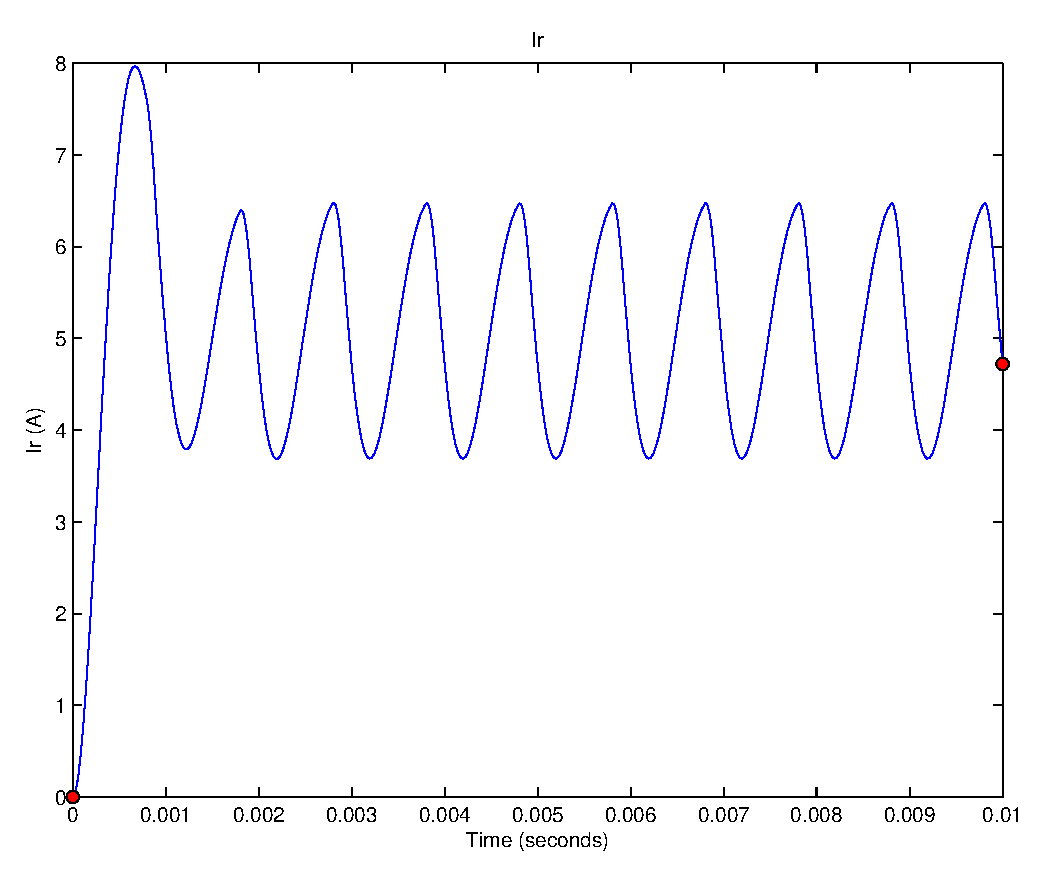
\includegraphics[width=\linewidth]{matlab/buck/b_ir2}
		\caption{Corrente no resistor}
	\end{subfigure}
	\caption{Curvas do resistor para conversor buck com indutância $\frac{L_b}{2}$}
	\label{fig:br2}
\end{figure}
\begin{figure}[H]
	\centering
	\begin{subfigure}[b]{0.4\linewidth}
		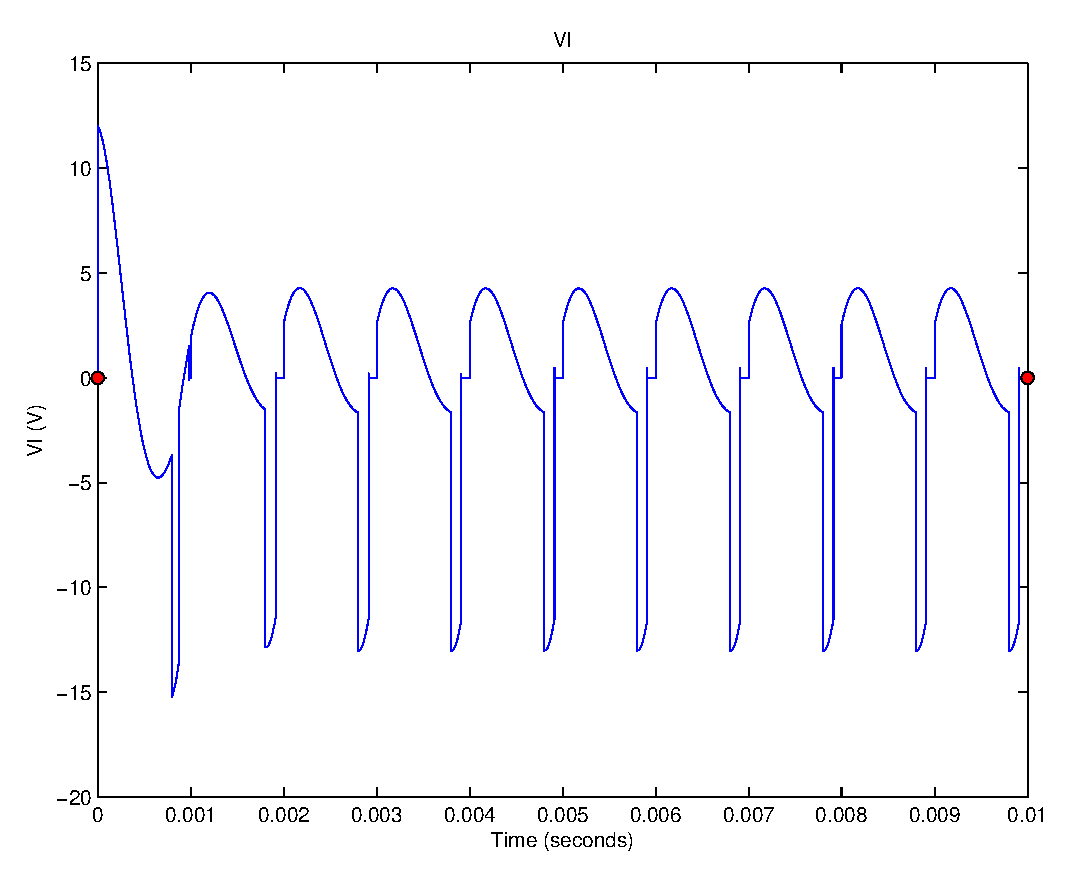
\includegraphics[width=\linewidth]{matlab/buck/b_vl2}
		\caption{Tensão no indutor}
	\end{subfigure}
	\begin{subfigure}[b]{0.4\linewidth}
		\centering
		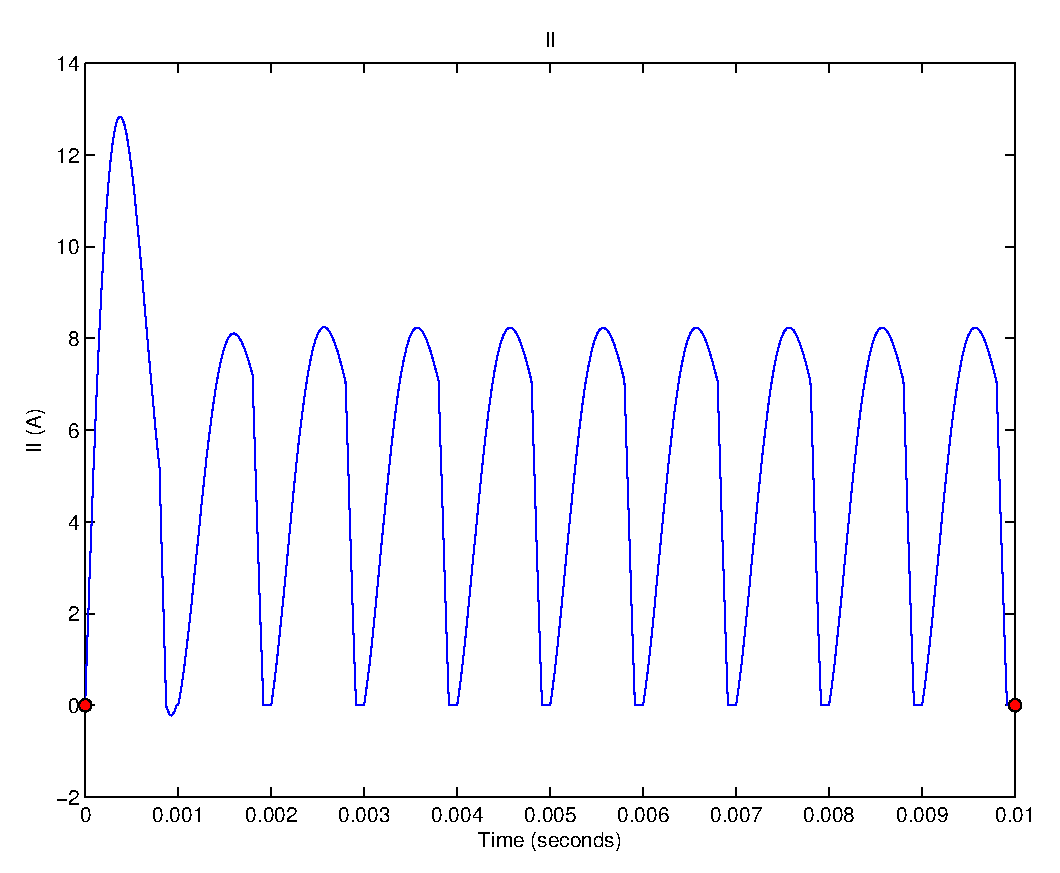
\includegraphics[width=\linewidth]{matlab/buck/b_il2}
		\caption{Corrente no indutor}
	\end{subfigure}
	\caption{Curvas do indutor para conversor buck com indutância $\frac{L_b}{2}$}
	\label{fig:bl2}
\end{figure}
\begin{figure}[H]
	\centering
	\begin{subfigure}[b]{0.4\linewidth}
		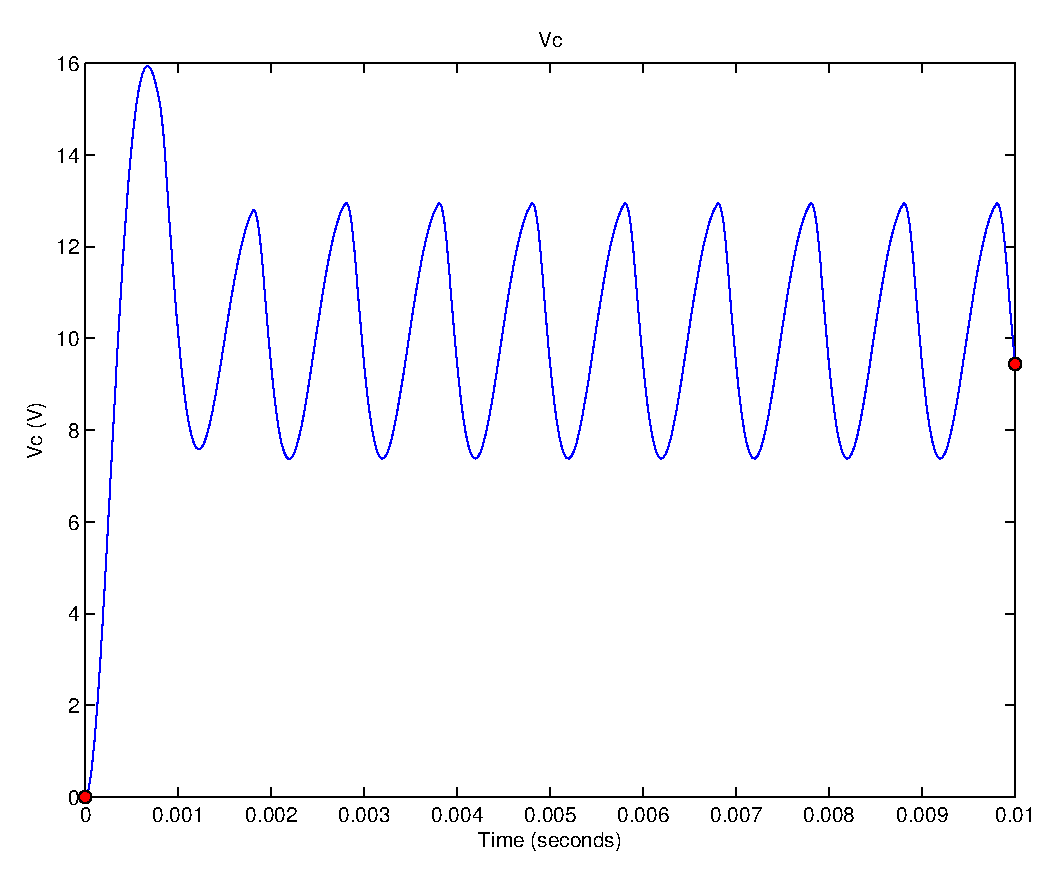
\includegraphics[width=\linewidth]{matlab/buck/b_vc2}
		\caption{Tensão no capacitor}
	\end{subfigure}
	\begin{subfigure}[b]{0.4\linewidth}
		\centering
		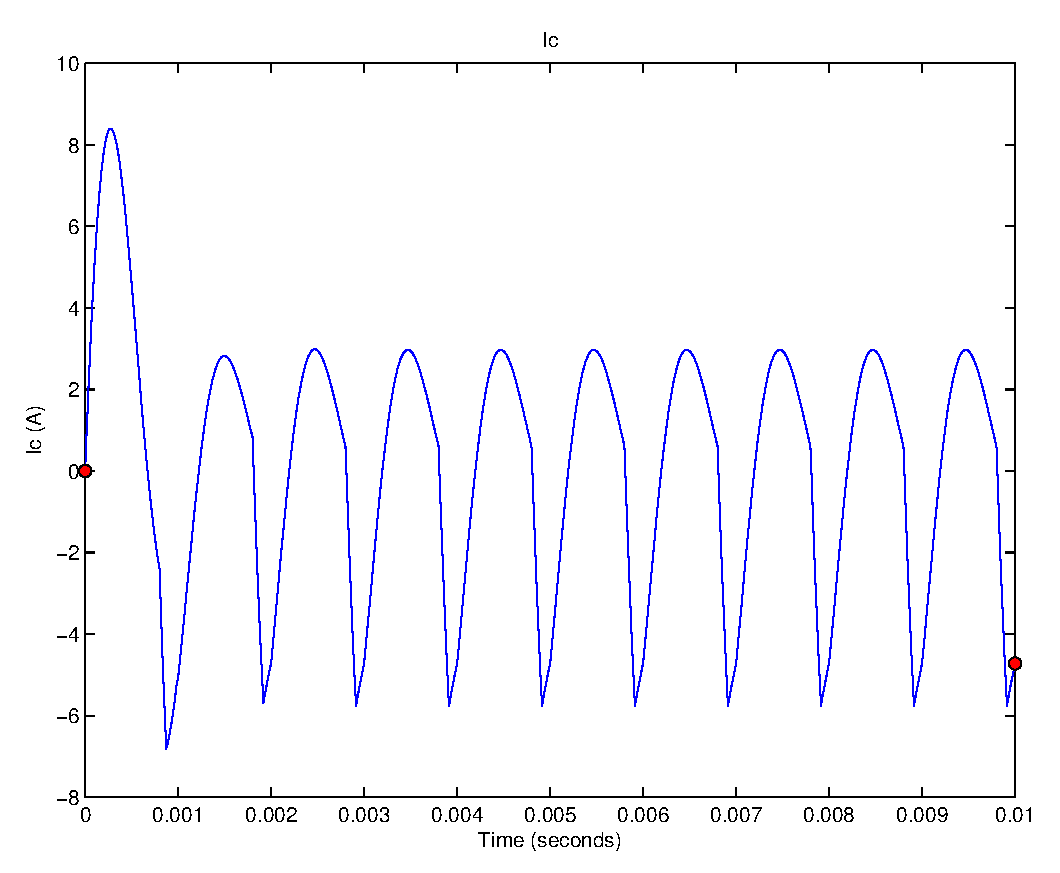
\includegraphics[width=\linewidth]{matlab/buck/b_ic2}
		\caption{Corrente no capacitor}
	\end{subfigure}
	\caption{Curvas do capacitor para conversor buck com indutância $\frac{L_b}{2}$}
	\label{fig:bc2}
\end{figure}
\begin{figure}[H]
	\centering
	\begin{subfigure}[b]{0.4\linewidth}
		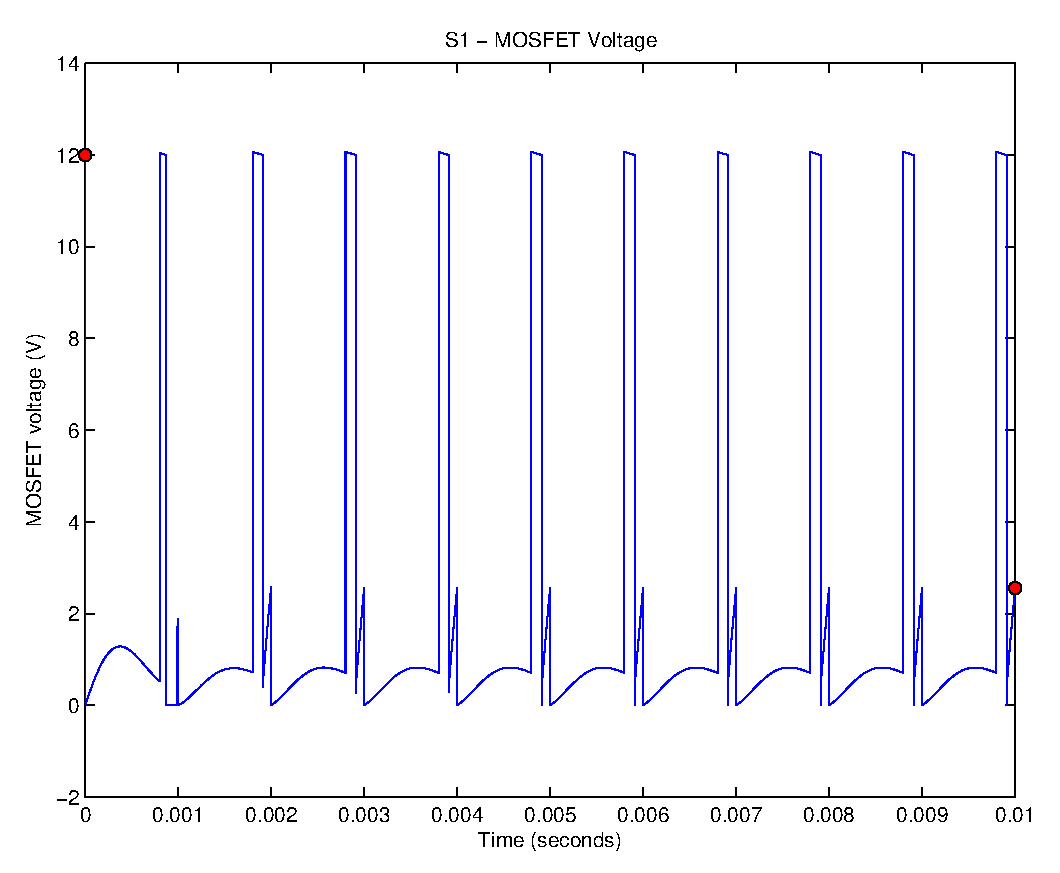
\includegraphics[width=\linewidth]{matlab/buck/r_s1v2}
		\caption{Tensão na chave S1}
	\end{subfigure}
	\begin{subfigure}[b]{0.4\linewidth}
		\centering
		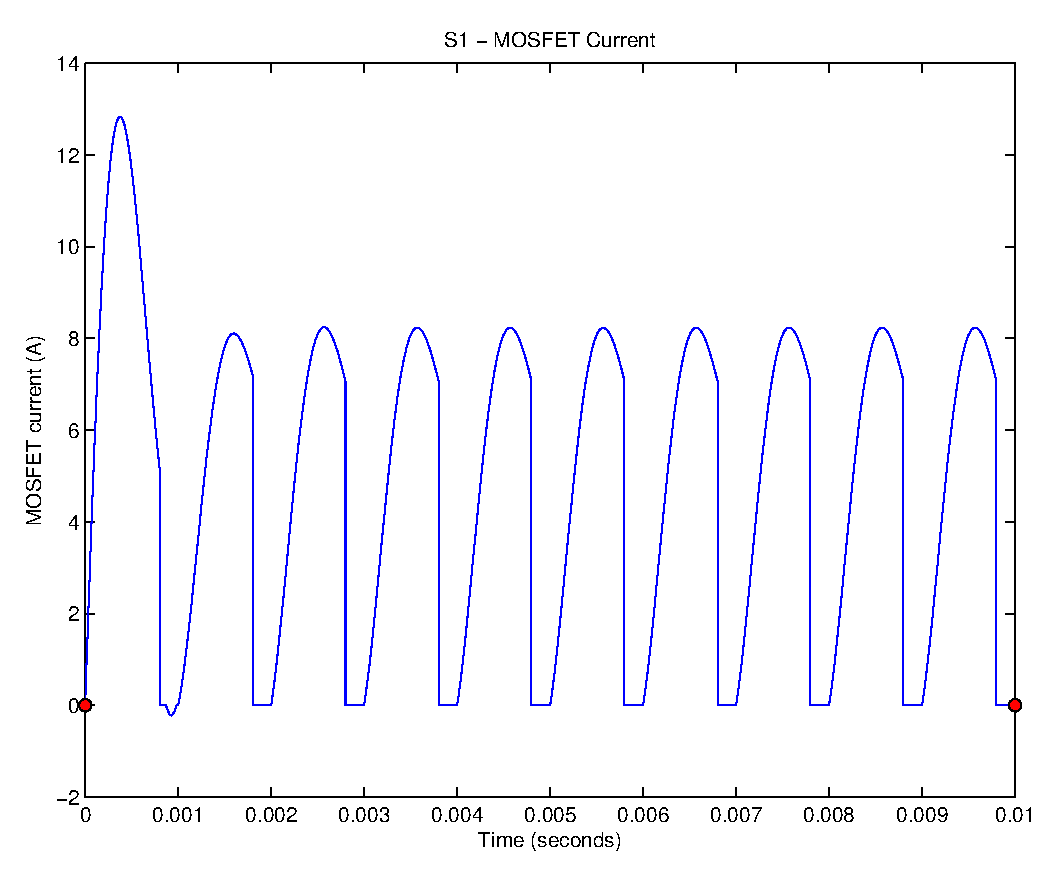
\includegraphics[width=\linewidth]{matlab/buck/r_s1i2}
		\caption{Corrente na chave S1}
	\end{subfigure}
	\caption{Curvas da chave S1 para conversor buck com indutância $\frac{L_b}{2}$}
	\label{fig:bs12}
\end{figure}
\begin{figure}[H]
	\centering
	\begin{subfigure}[b]{0.4\linewidth}
		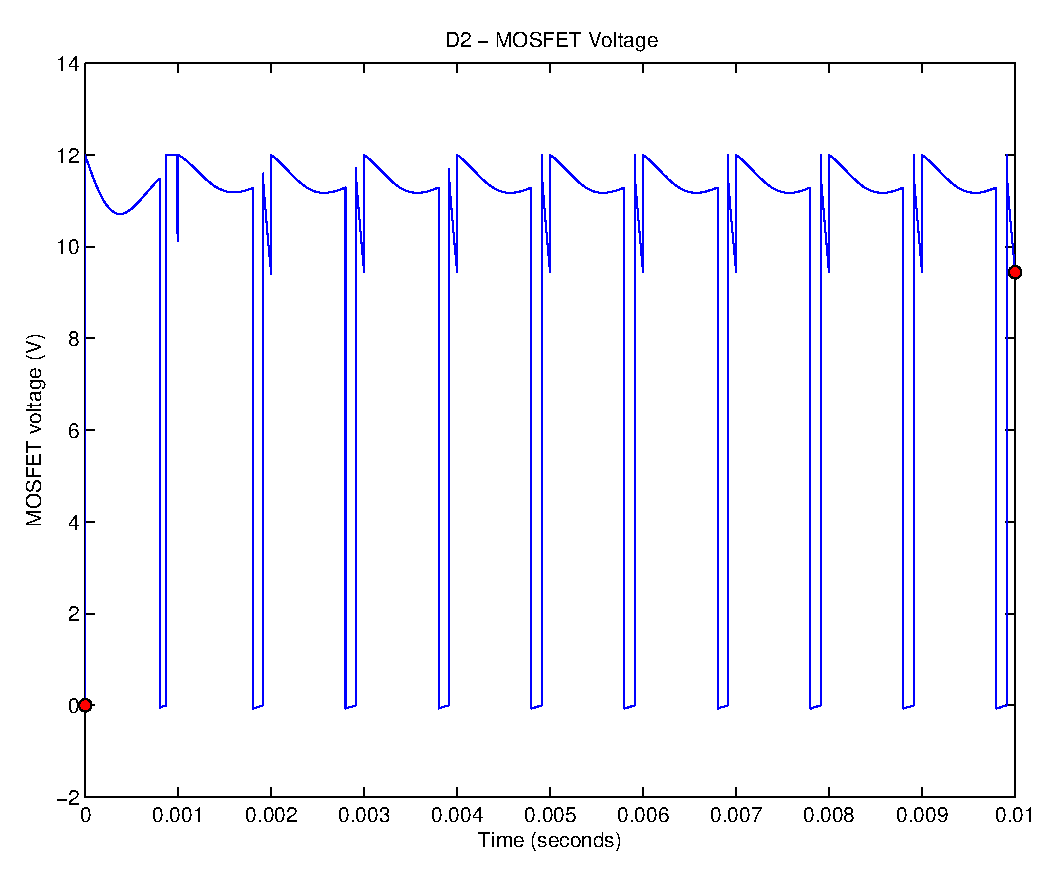
\includegraphics[width=\linewidth]{matlab/buck/r_d2v2}
		\caption{Tensão no diodo D2}
	\end{subfigure}
	\begin{subfigure}[b]{0.4\linewidth}
		\centering
		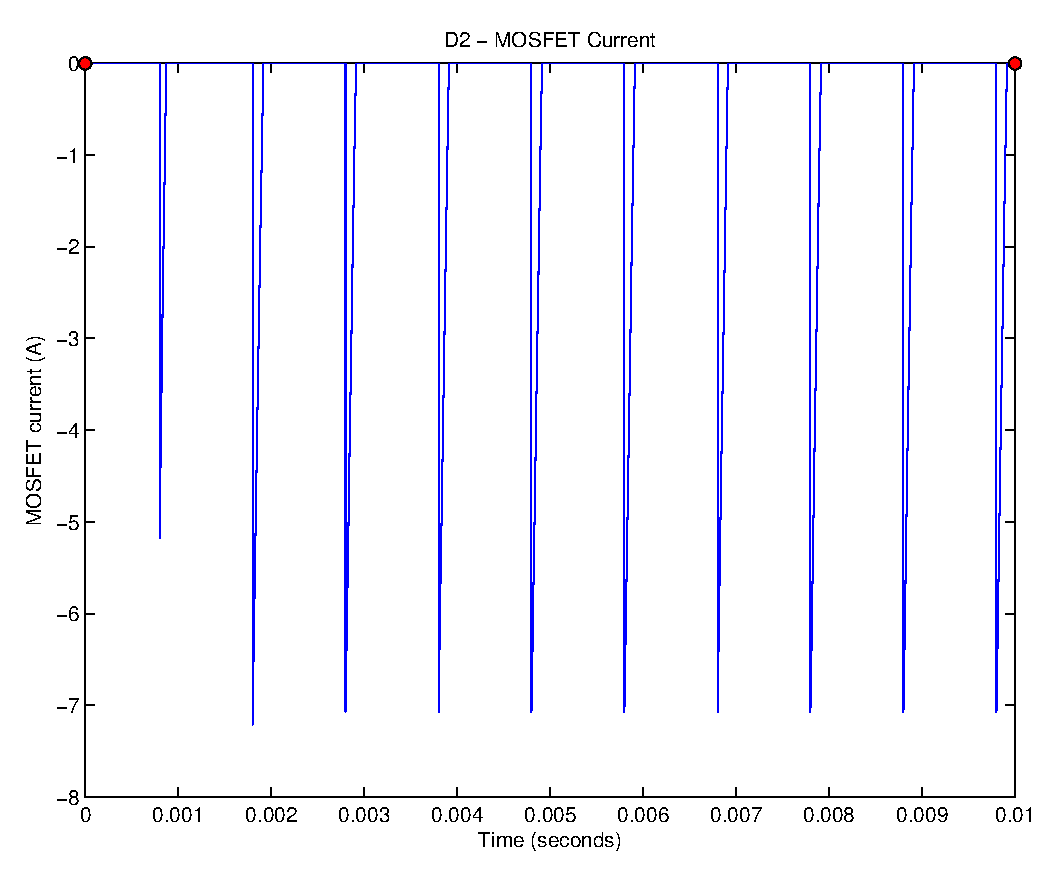
\includegraphics[width=\linewidth]{matlab/buck/r_d2i2}
		\caption{Corrente no diodo D2}
	\end{subfigure}
	\caption{Curvas do diodo D2 para conversor buck com indutância $\frac{L_b}{2}$}
	\label{fig:bd22}
\end{figure}

%TODO ANALISAR

Por fim voltamos a nossa indutância original porém retiramos o filtro capacitivo, encontramos então a curva de tensão sobre o resistor apresentada na figura \ref{fig:br3}.
\begin{figure}[H]
	\centering
	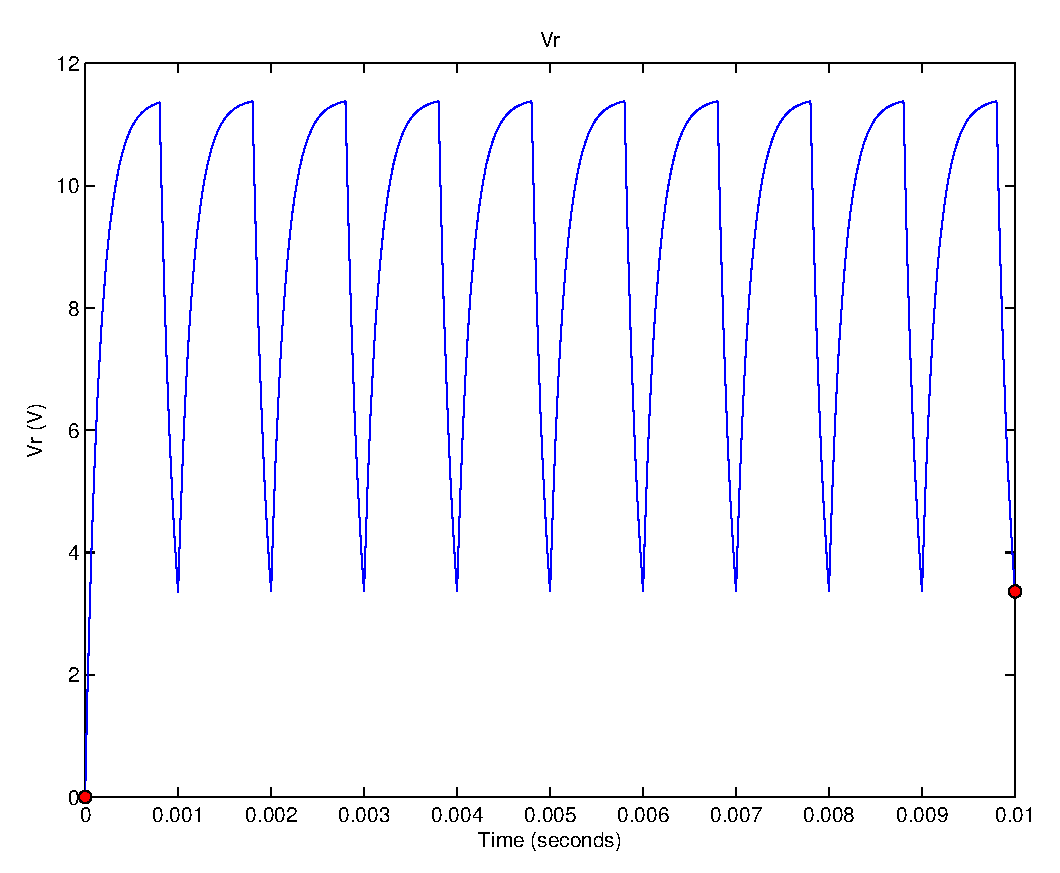
\includegraphics[width=0.7\linewidth]{matlab/buck/b_vr3}
	\caption{Tensão no resistor para conversor buck sem filtro capacitivo}
	\label{fig:br3}
\end{figure}

%TODO Concluir

\section{Conversor Boost}
Através do Simulink implementamos o conversor step-up detalhado na figura \ref{fig:bosim}.
\begin{figure}[H]
	\centering
	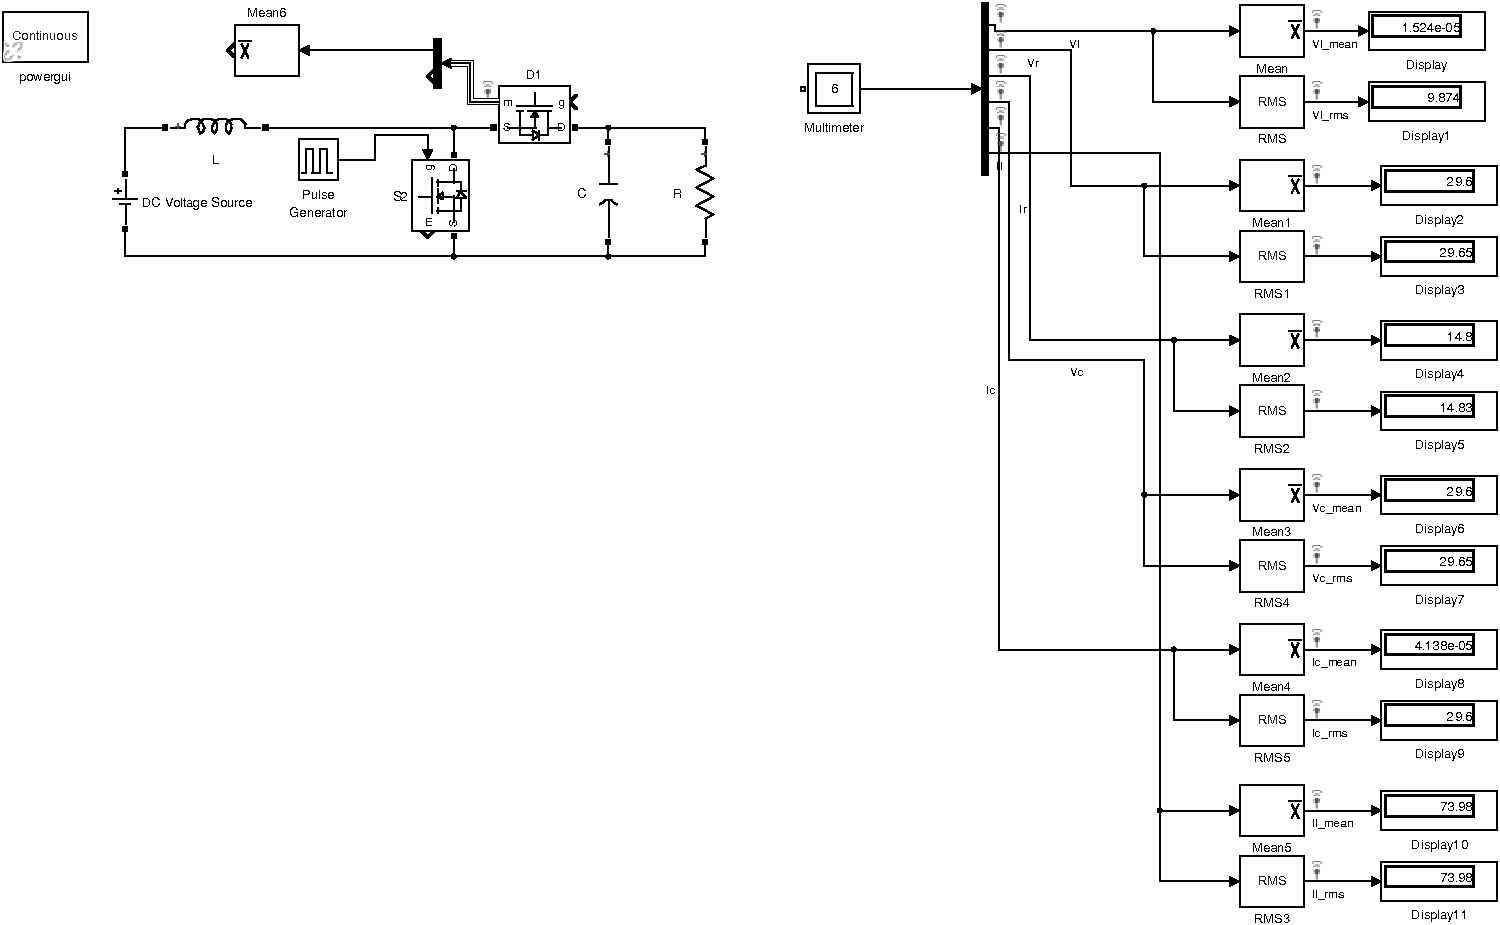
\includegraphics[width=\linewidth]{matlab/boost/bsim}
	\caption{Esquema para simulação do conversor boost}
	\label{fig:bosim}
\end{figure}
Conforme detalhados no roteiro, setamos os parâmetros $R$ = $2\Omega$, $C$ = $220\mu F$, $L$ = $330\mu H$ e simulamos o sistema com uma frequência $f$ = $10kHz$ e duty-cicle de 80\% na chave S2.
Extraímos dessa simulação as curvas de tensão e corrente na carga (figura \ref{fig:bor}), no indutor (figura \ref{fig:bol}), no capacitor (figura \ref{fig:boc}), na chave S2 (figura \ref{fig:bos2}) e no diodo D1 (figura \ref{fig:bod1}).
\begin{figure}[H]
	\centering
	\begin{subfigure}[b]{0.4\linewidth}
		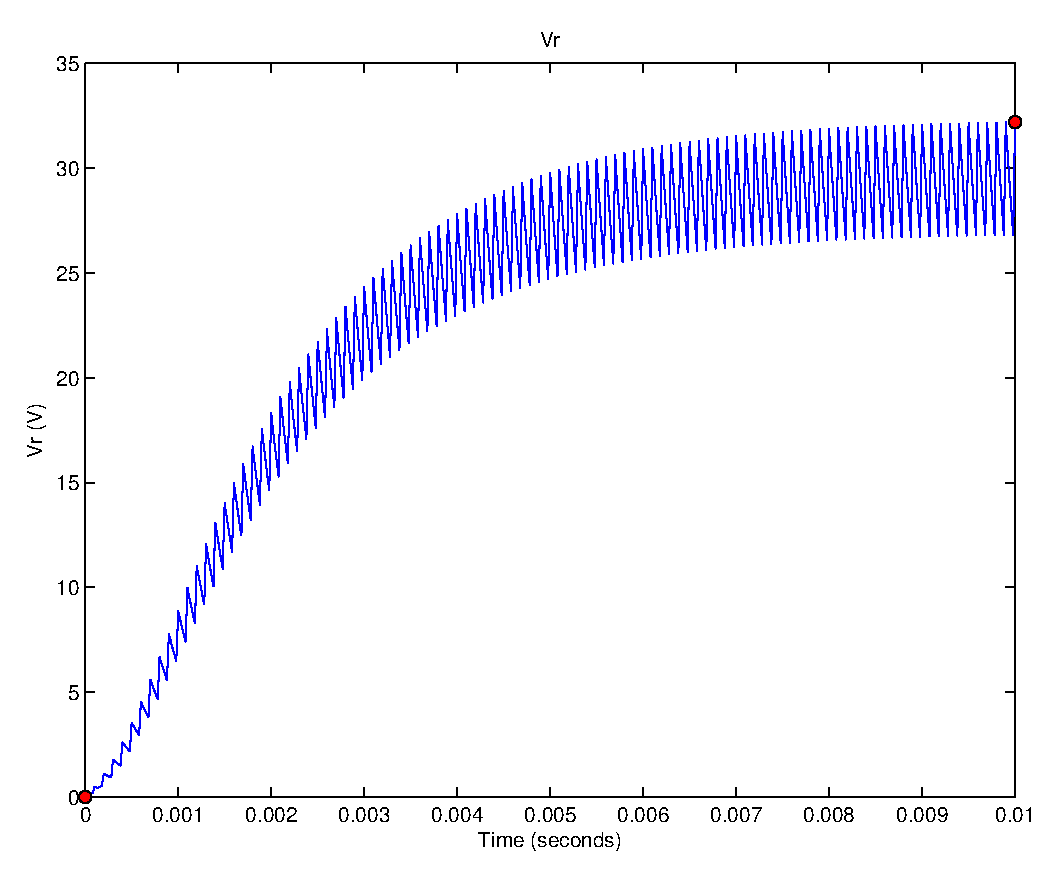
\includegraphics[width=\linewidth]{matlab/boost/b_vr}
		\caption{Tensão no resistor}
	\end{subfigure}
	\begin{subfigure}[b]{0.4\linewidth}
		\centering
		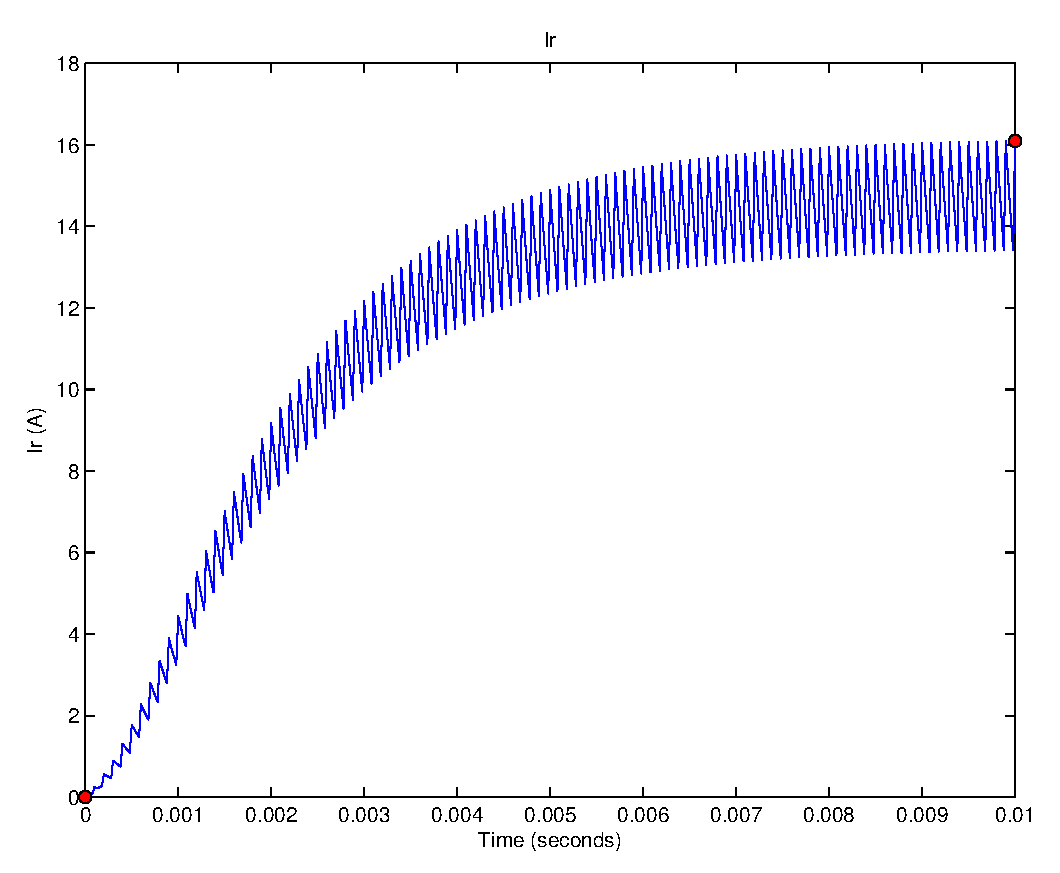
\includegraphics[width=\linewidth]{matlab/boost/b_ir}
		\caption{Corrente no resistor}
	\end{subfigure}
	\begin{subfigure}[b]{0.4\linewidth}
		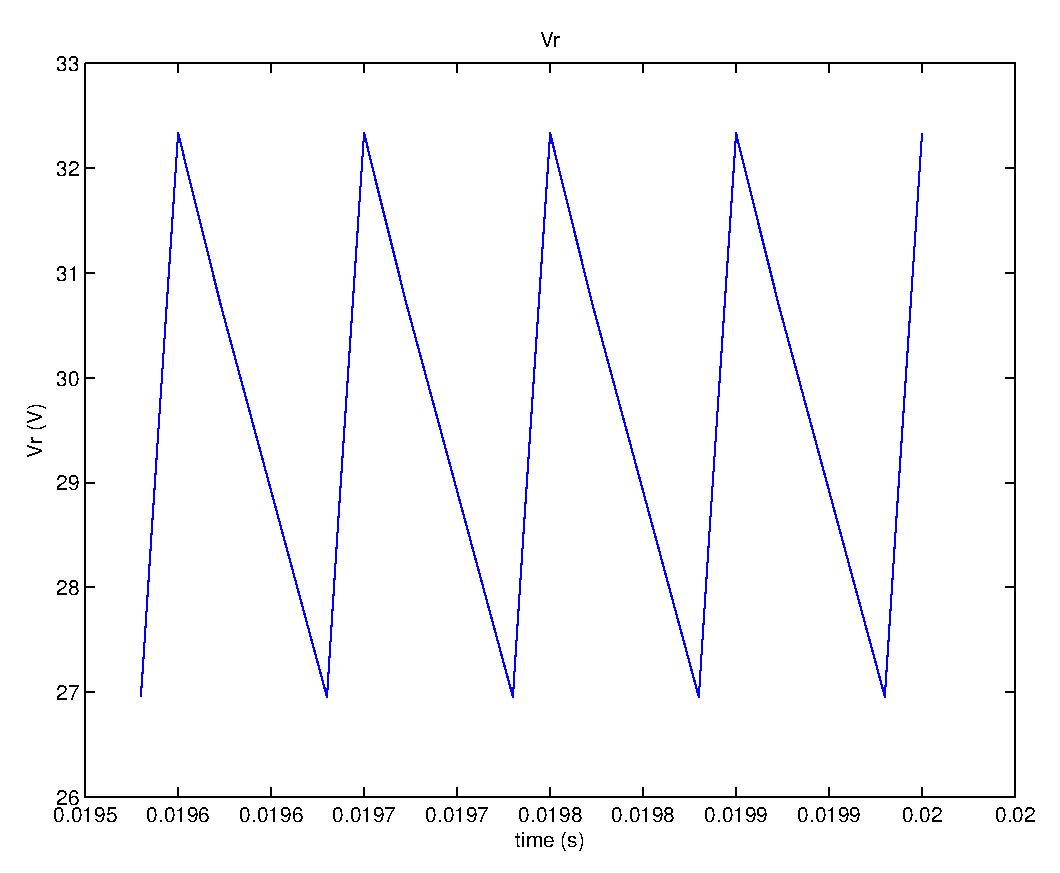
\includegraphics[width=\linewidth]{matlab/boost/b_vrst}
		\caption{Tensão no resistor após equilíbrio}
	\end{subfigure}
	\begin{subfigure}[b]{0.4\linewidth}
		\centering
		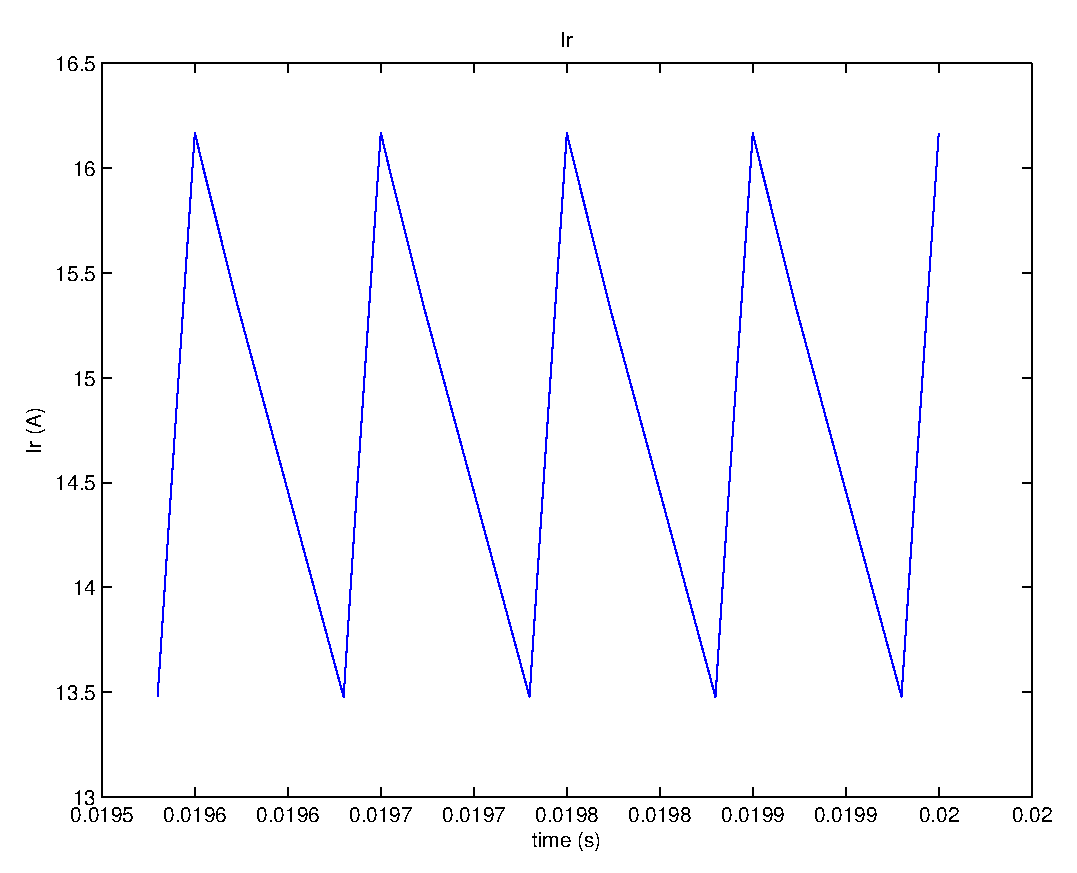
\includegraphics[width=\linewidth]{matlab/boost/b_irst}
		\caption{Corrente no resistor após equilíbrio}
	\end{subfigure}
	\caption{Curvas do resistor para conversor boost}
	\label{fig:bor}
\end{figure}
\begin{figure}[H]
	\centering
	\begin{subfigure}[b]{0.4\linewidth}
		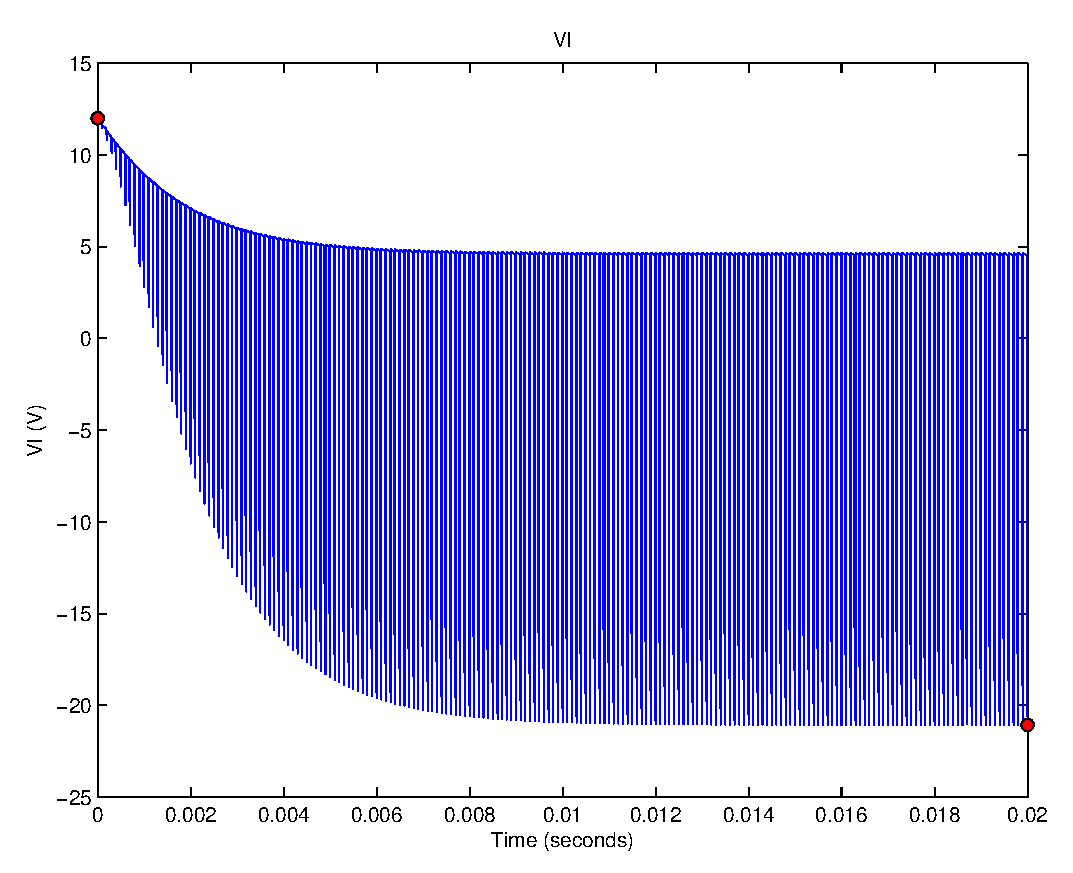
\includegraphics[width=\linewidth]{matlab/boost/b_vl}
		\caption{Tensão no indutor}
	\end{subfigure}
	\begin{subfigure}[b]{0.4\linewidth}
		\centering
		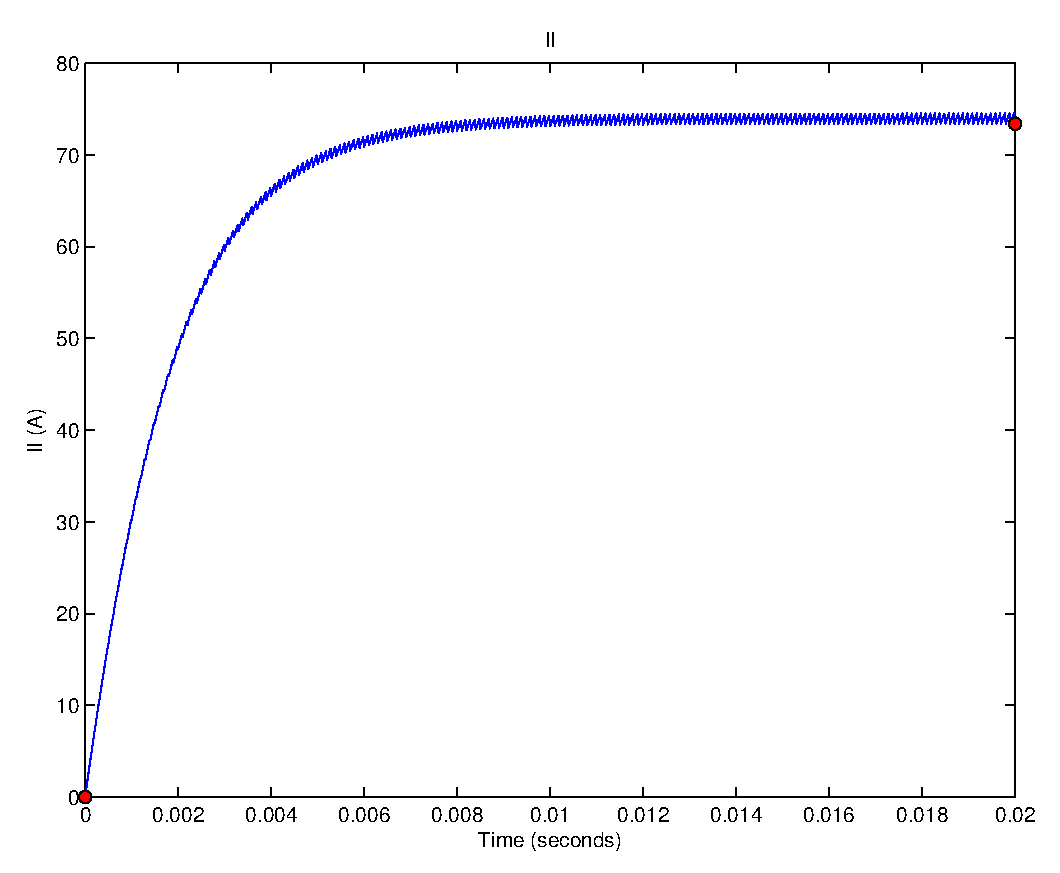
\includegraphics[width=\linewidth]{matlab/boost/b_il}
		\caption{Corrente no indutor}
	\end{subfigure}
	\begin{subfigure}[b]{0.4\linewidth}
		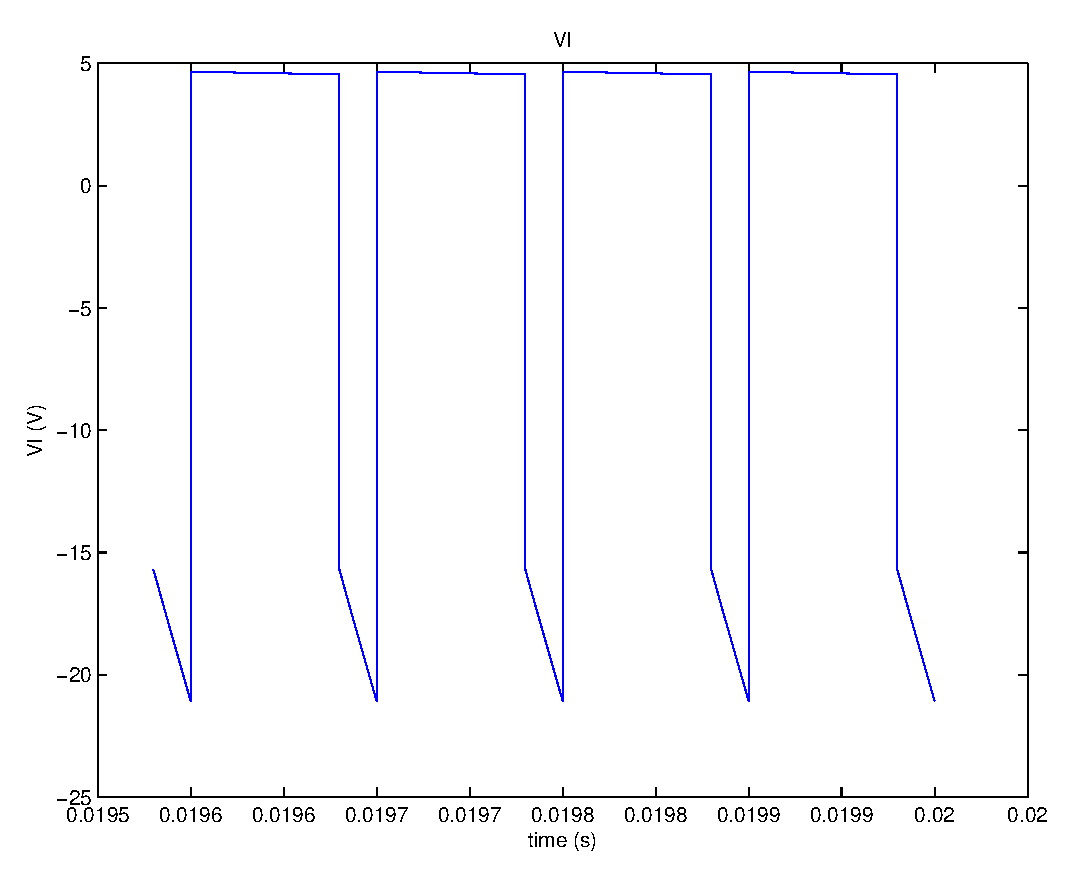
\includegraphics[width=\linewidth]{matlab/boost/b_vlst}
		\caption{Tensão no indutor após equilíbrio}
	\end{subfigure}
	\begin{subfigure}[b]{0.4\linewidth}
		\centering
		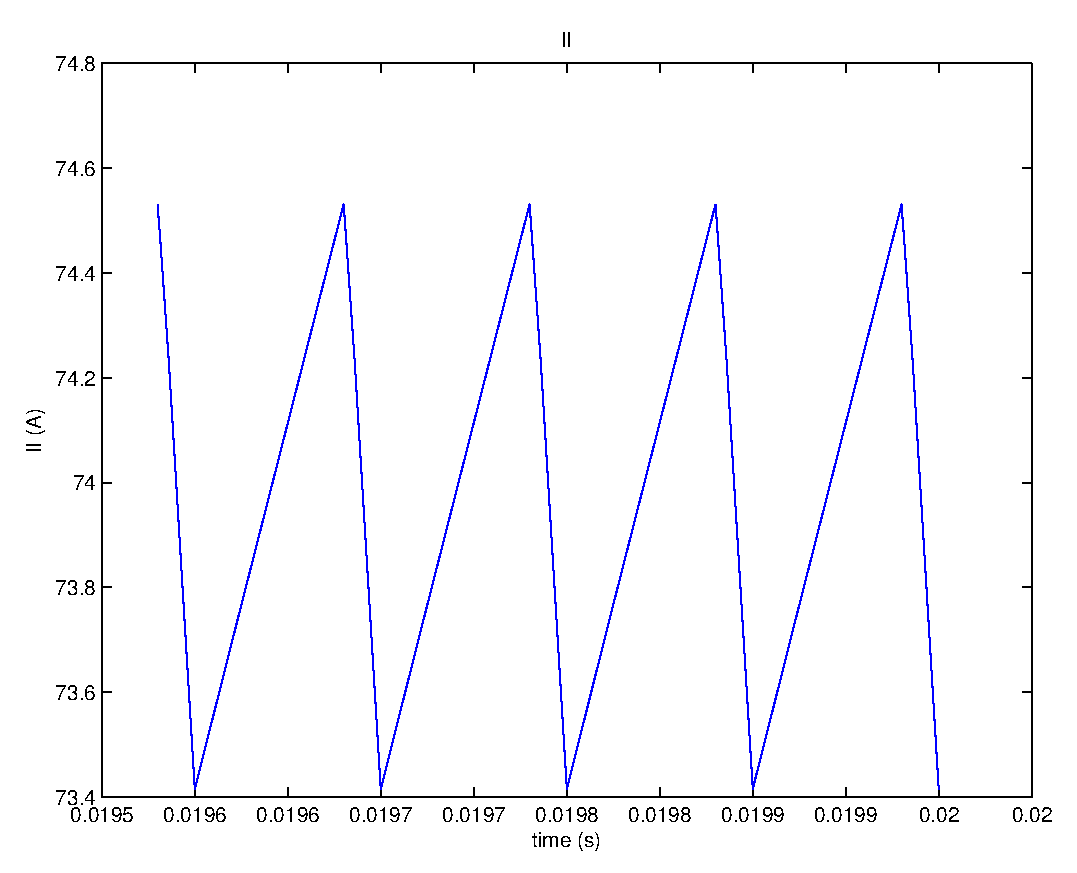
\includegraphics[width=\linewidth]{matlab/boost/b_ilst}
		\caption{Corrente no indutor após equilíbrio}
	\end{subfigure}
	\caption{Curvas do indutor para conversor boost}
	\label{fig:bol}
\end{figure}
\begin{figure}[H]
	\centering
	\begin{subfigure}[b]{0.4\linewidth}
		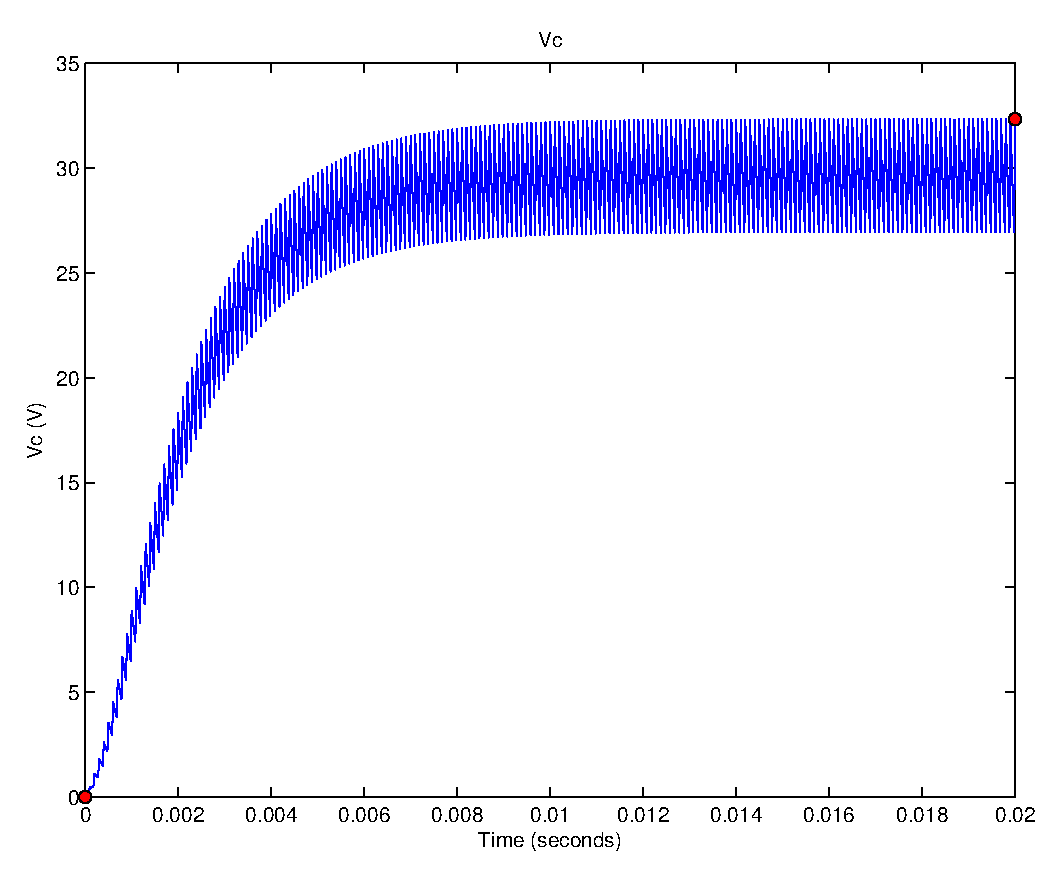
\includegraphics[width=\linewidth]{matlab/boost/b_vc}
		\caption{Tensão no capacitor}
	\end{subfigure}
	\begin{subfigure}[b]{0.4\linewidth}
		\centering
		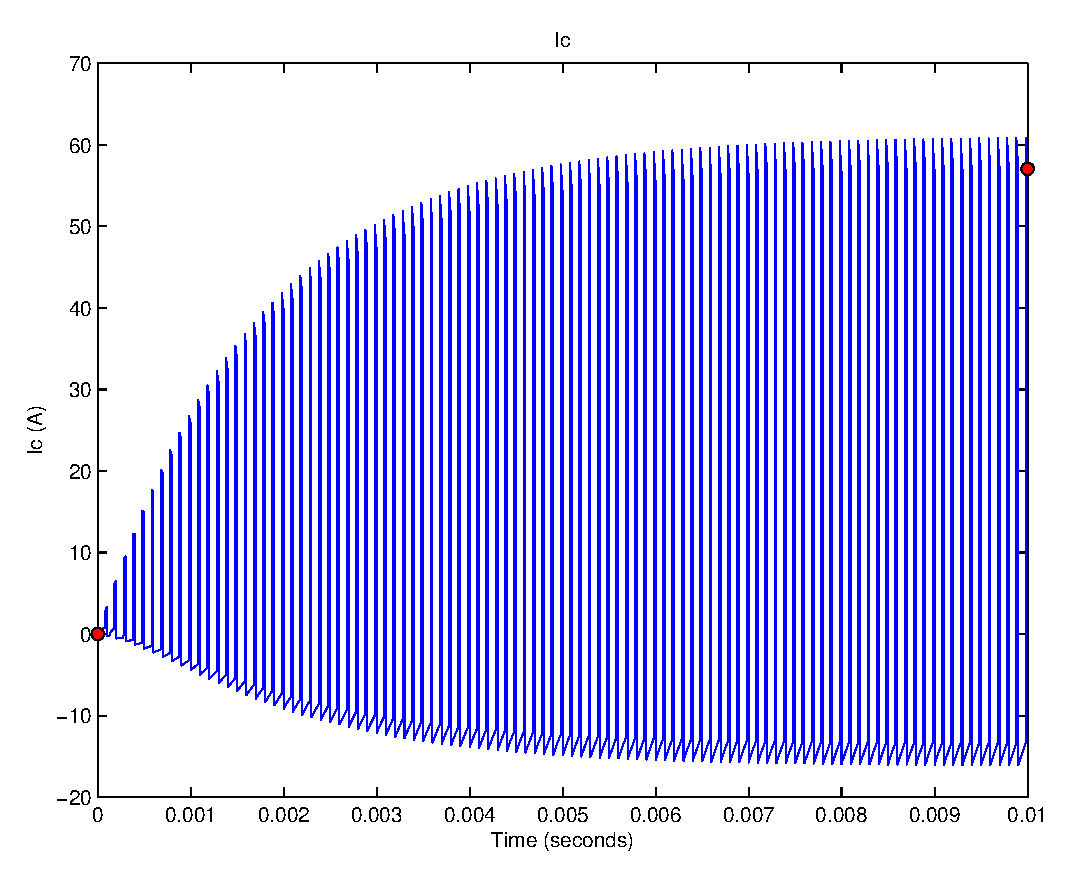
\includegraphics[width=\linewidth]{matlab/boost/b_ic}
		\caption{Corrente no capacitor}
	\end{subfigure}
	\begin{subfigure}[b]{0.4\linewidth}
		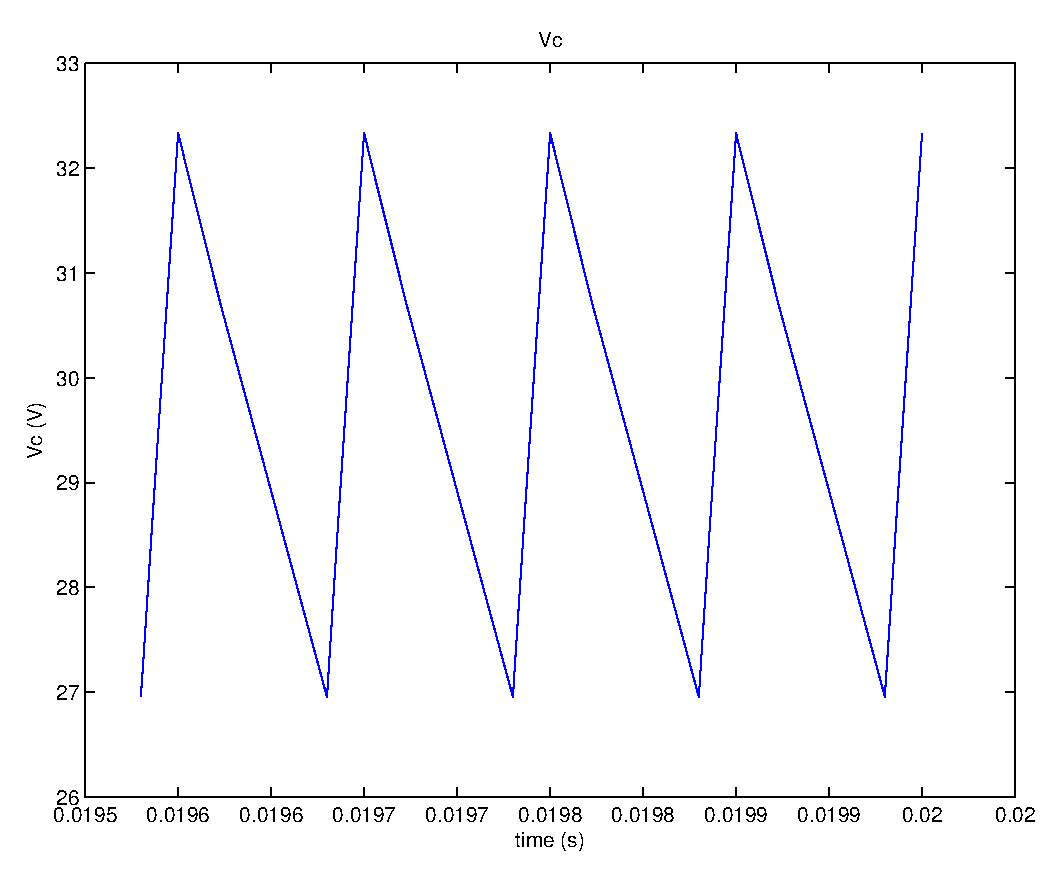
\includegraphics[width=\linewidth]{matlab/boost/b_vcst}
		\caption{Tensão no capacitor após equilíbrio}
	\end{subfigure}
	\begin{subfigure}[b]{0.4\linewidth}
		\centering
		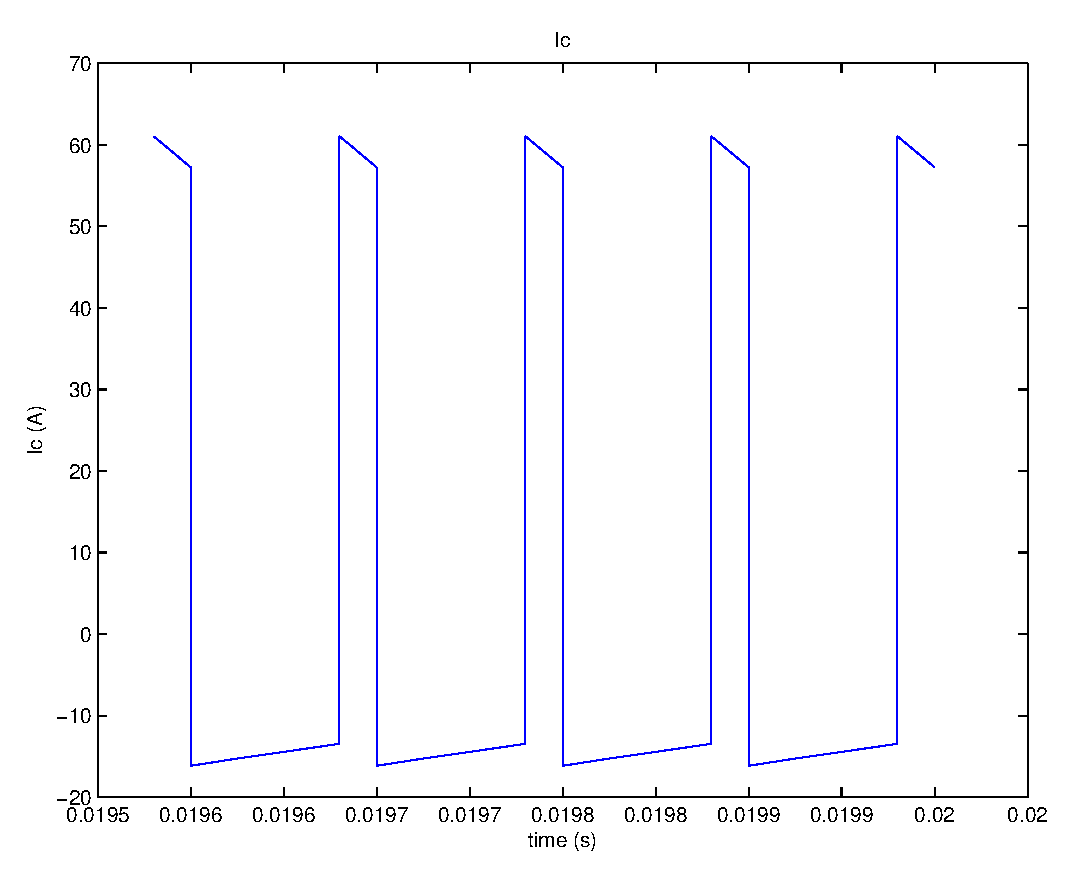
\includegraphics[width=\linewidth]{matlab/boost/b_icst}
		\caption{Corrente no capacitor após equilíbrio}
	\end{subfigure}
	\caption{Curvas do capacitor para conversor boost}
	\label{fig:boc}
\end{figure}
\begin{figure}[H]
	\centering
	\begin{subfigure}[b]{0.4\linewidth}
		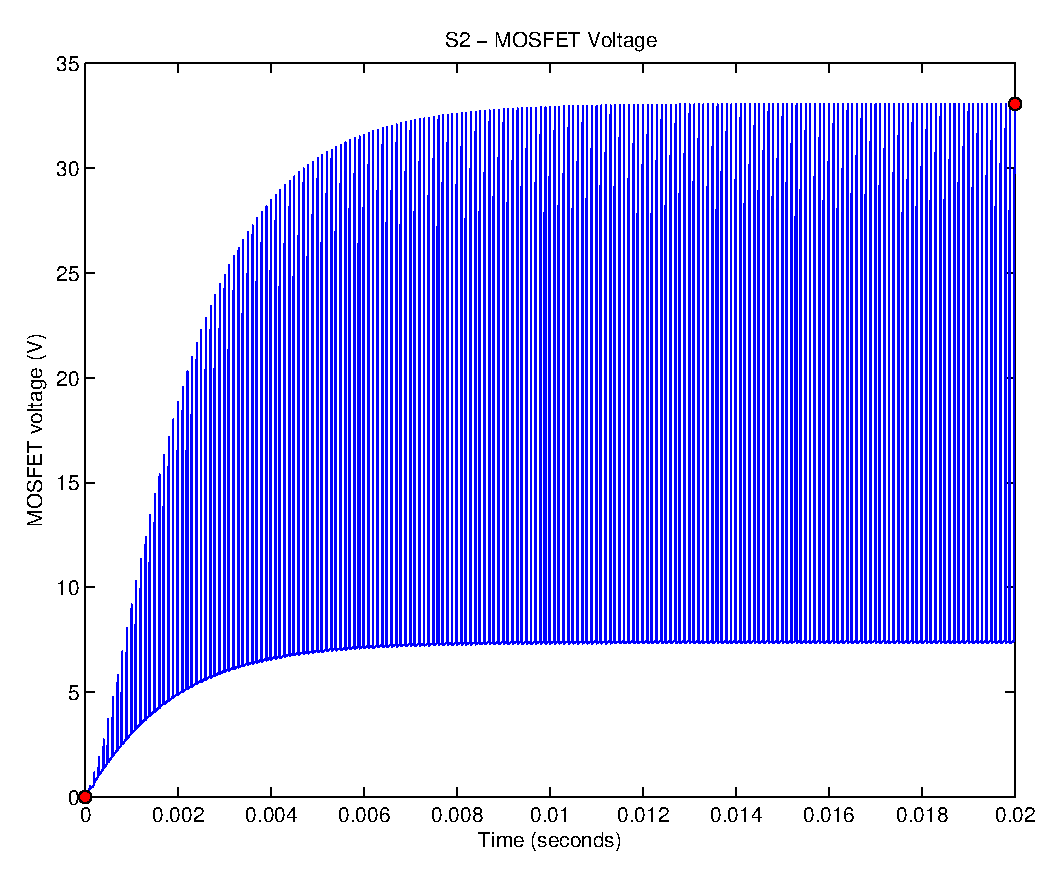
\includegraphics[width=\linewidth]{matlab/boost/r_s2v}
		\caption{Tensão na chave S2}
	\end{subfigure}
	\begin{subfigure}[b]{0.4\linewidth}
		\centering
		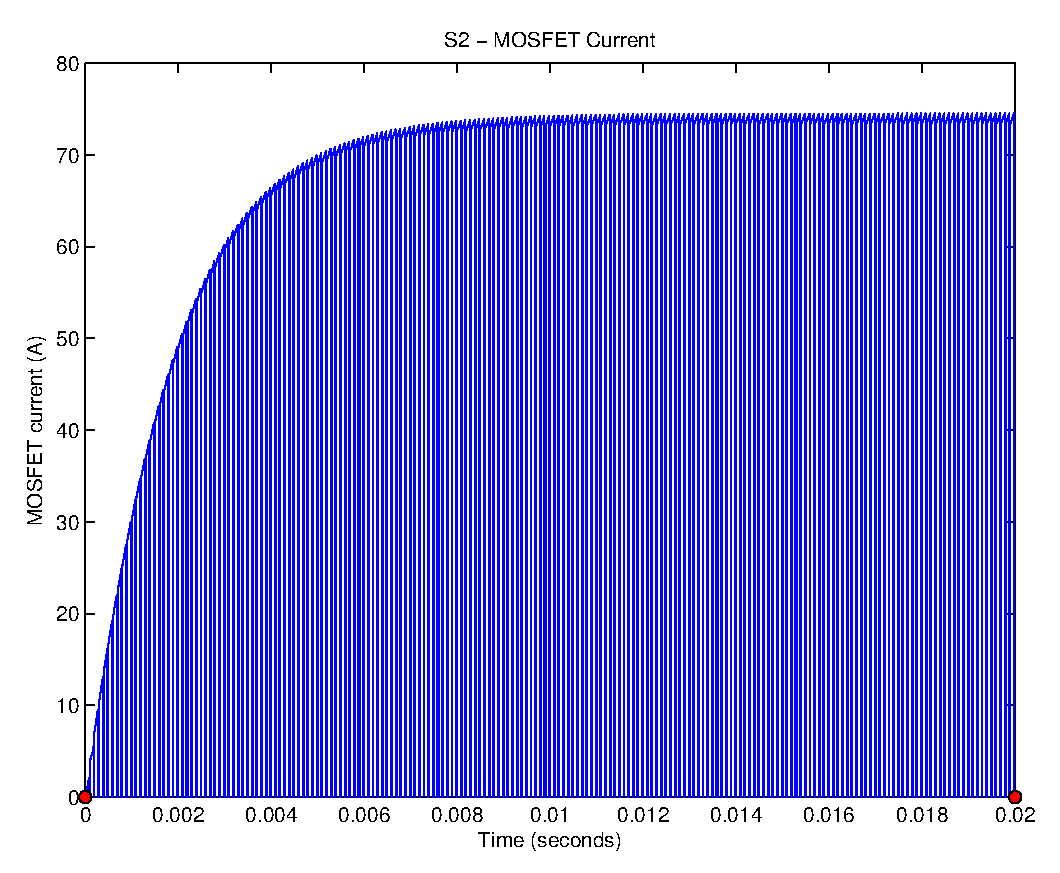
\includegraphics[width=\linewidth]{matlab/boost/r_s2i}
		\caption{Corrente na chave S2}
	\end{subfigure}
	\begin{subfigure}[b]{0.4\linewidth}
		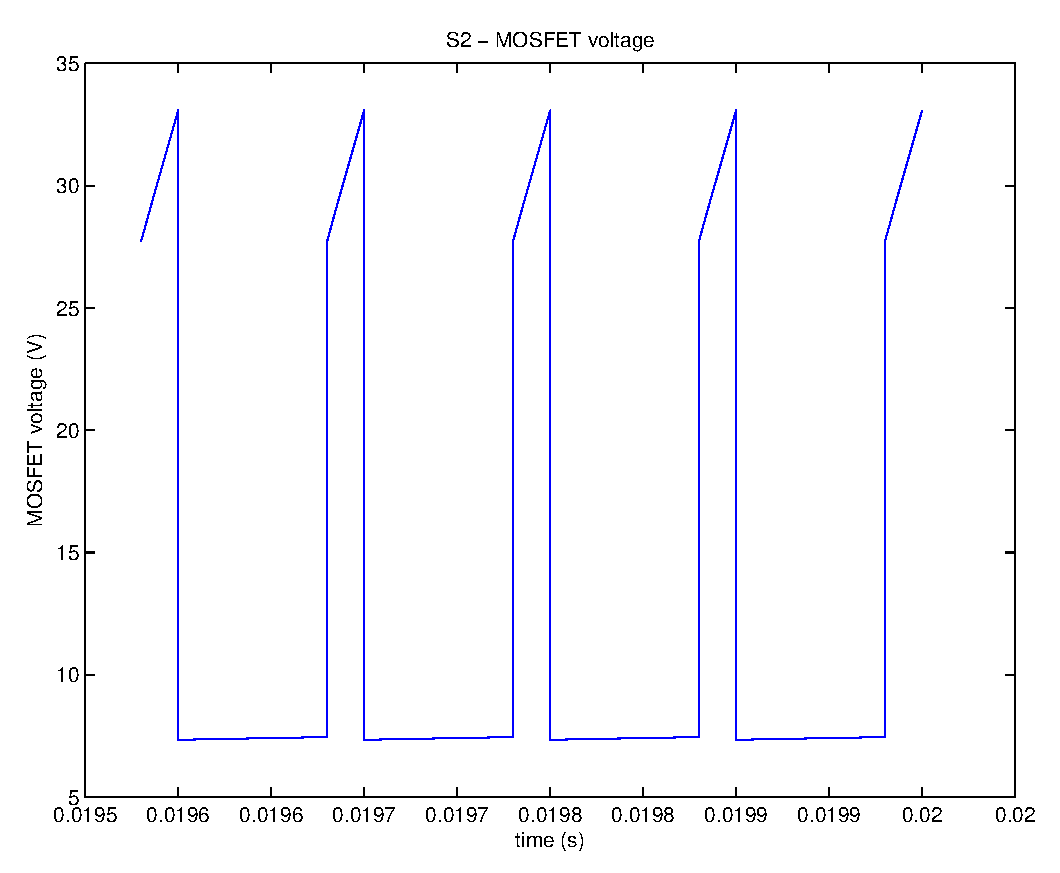
\includegraphics[width=\linewidth]{matlab/boost/r_s2vst}
		\caption{Tensão na chave S2 após equilíbrio}
	\end{subfigure}
	\begin{subfigure}[b]{0.4\linewidth}
		\centering
		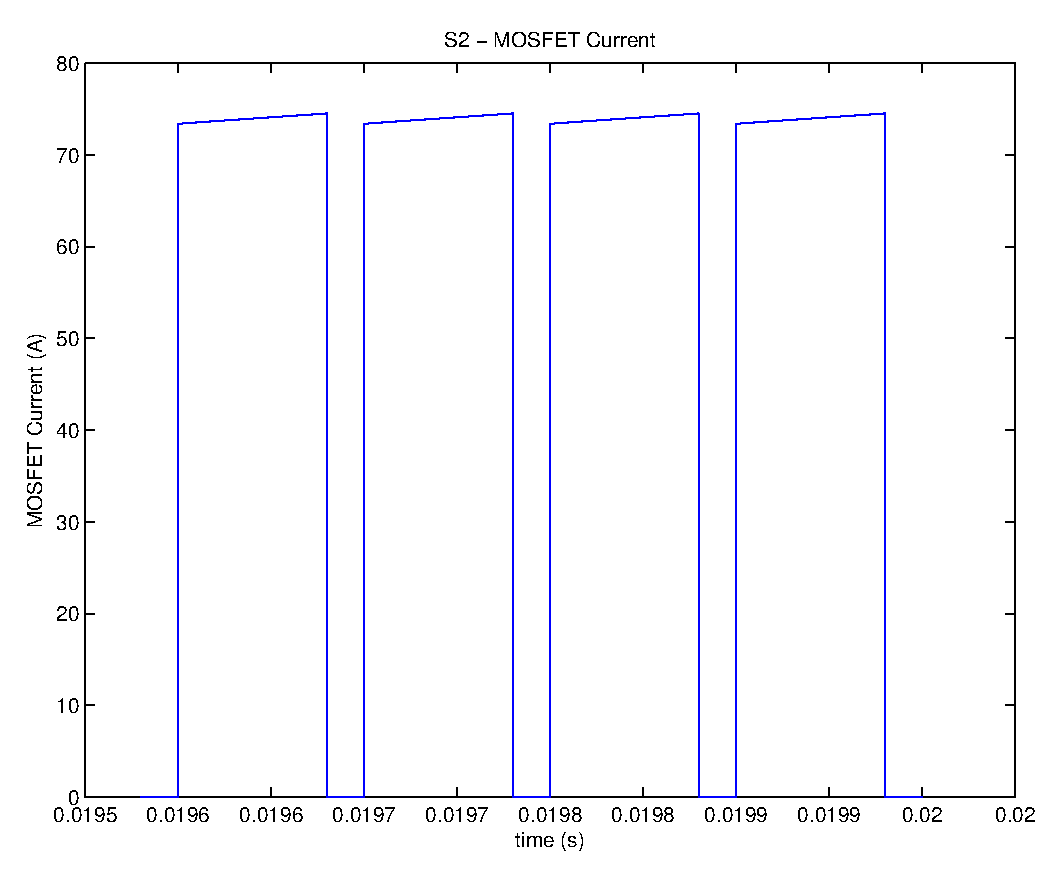
\includegraphics[width=\linewidth]{matlab/boost/r_s2ist}
		\caption{Corrente na chave S2 após equilíbrio}
	\end{subfigure}
	\caption{Curvas da chave S2 para conversor boost}
	\label{fig:bos2}
\end{figure}
\begin{figure}[H]
	\centering
	\begin{subfigure}[b]{0.4\linewidth}
		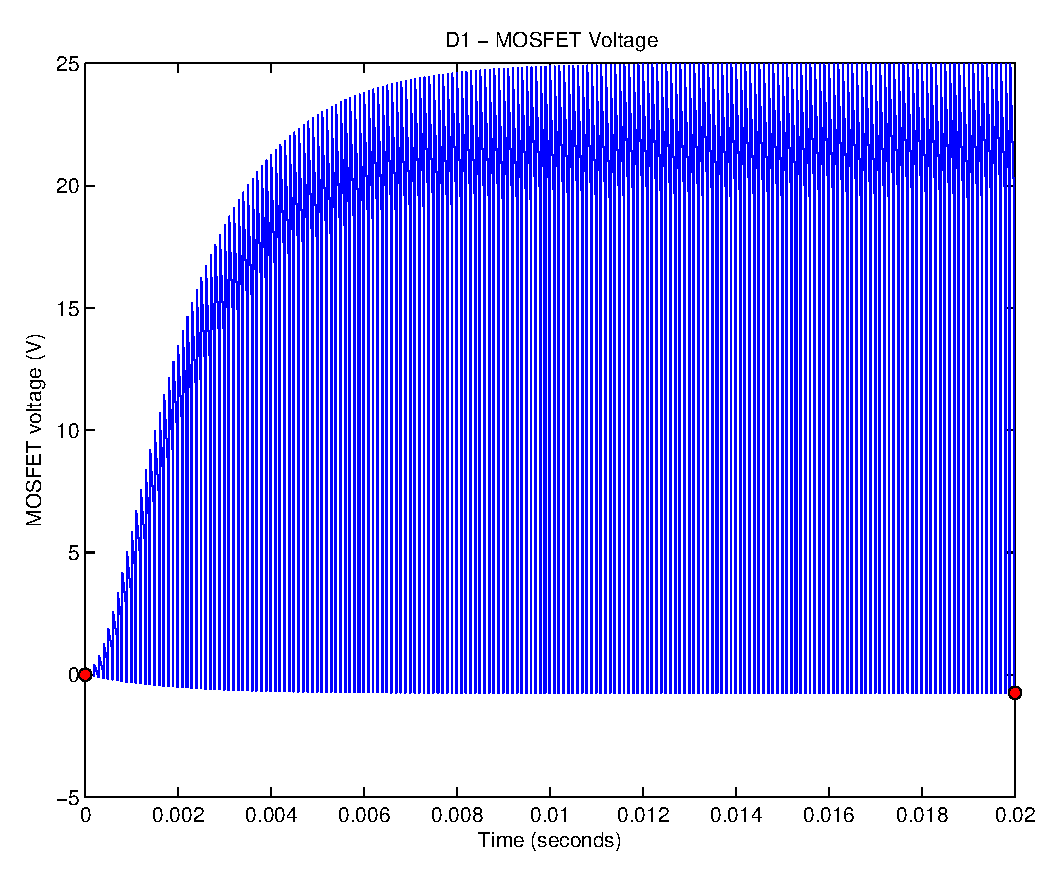
\includegraphics[width=\linewidth]{matlab/boost/r_d1v}
		\caption{Tensão no diodo D1}
	\end{subfigure}
	\begin{subfigure}[b]{0.4\linewidth}
		\centering
		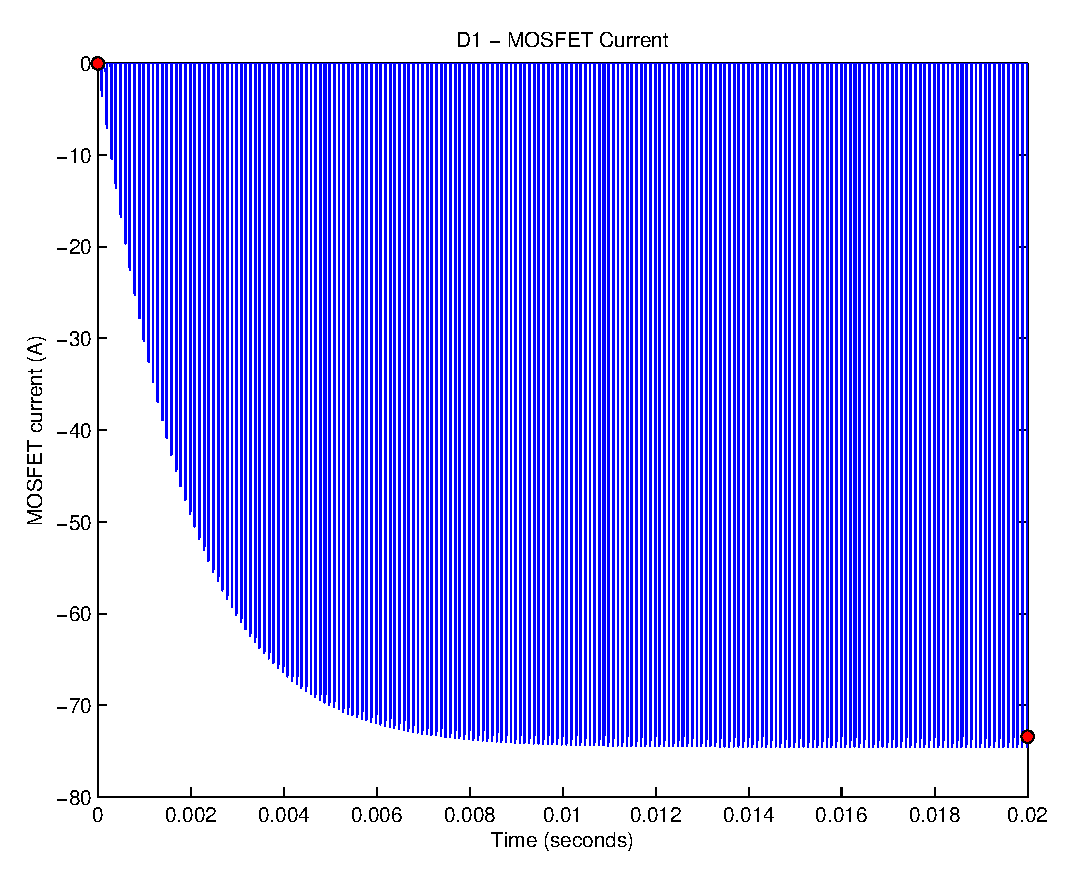
\includegraphics[width=\linewidth]{matlab/boost/r_d1i}
		\caption{Corrente no diodo D1}
	\end{subfigure}
		\begin{subfigure}[b]{0.4\linewidth}
			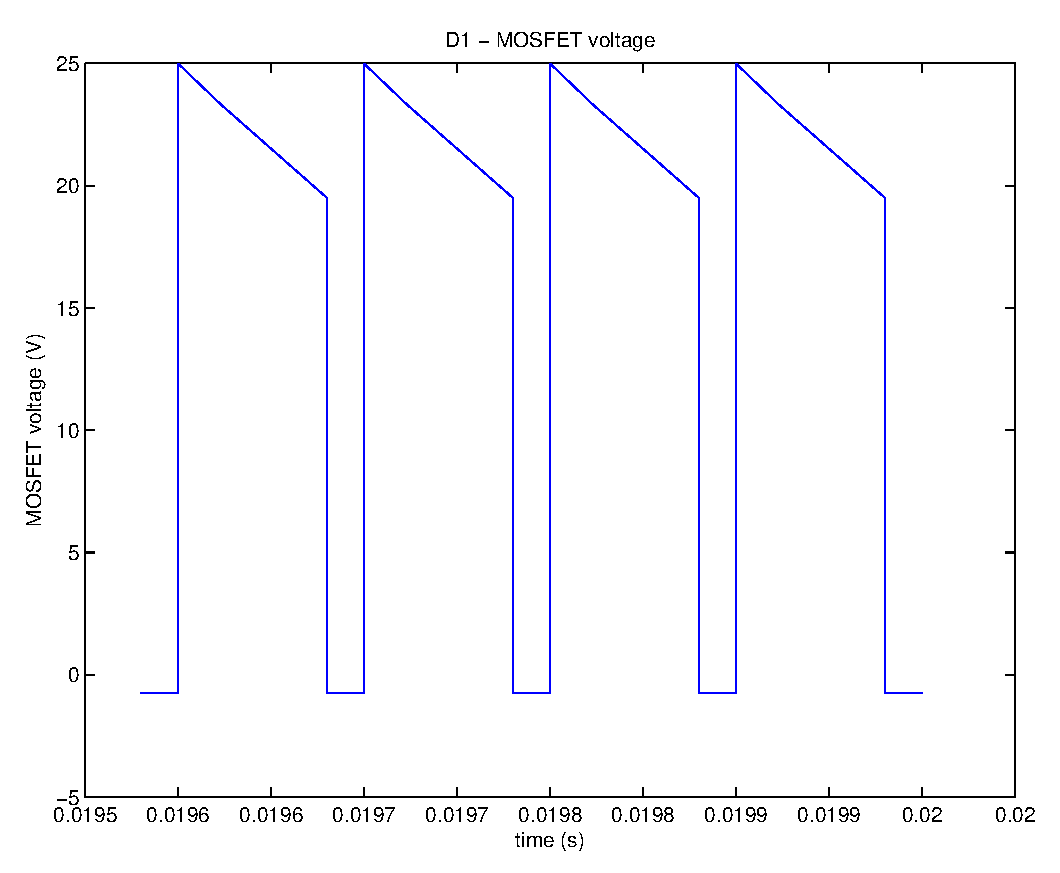
\includegraphics[width=\linewidth]{matlab/boost/r_d1vst}
			\caption{Tensão no diodo D1 após equilíbrio}
		\end{subfigure}
		\begin{subfigure}[b]{0.4\linewidth}
			\centering
			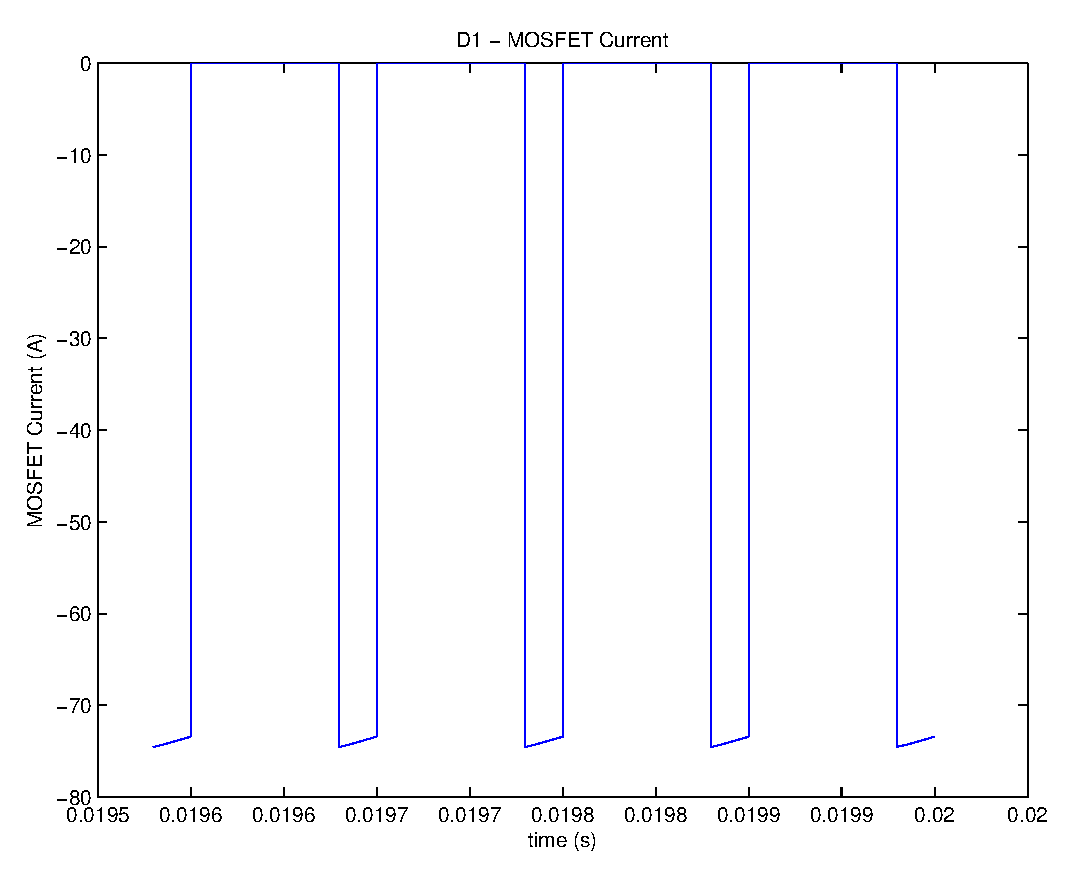
\includegraphics[width=\linewidth]{matlab/boost/r_d1ist}
			\caption{Corrente no diodo D1 após equilíbrio}
		\end{subfigure}
	\caption{Curvas do diodo D1 para conversor boost}
	\label{fig:bod1}
\end{figure}

Medimos as tensões média e efetiva no resistor, obtendo os seguintes valores:
\begin{equation}
\overline{Vr} = 29.6\ V
\end{equation}
\begin{equation}
Vr_{rms} = 29.65\ V
\end{equation}

Conforme podemos ver analisando as curvas, %TODO

Podemos calcular a tensão média teórica sobre a carga através da equação \ref{eq:bomean}
%TODO
\begin{equation}
\overline{Vr} = 
\label{eq:bomean}
\end{equation}

Variamos então o valor do duty-cicle entre 0 e 100\% e encontramos a tensão média sobre a carga. Comparamos esse valor com o valor teórico esperado na figura \ref{fig:bovrxd}
\begin{figure}[H]
	\centering
	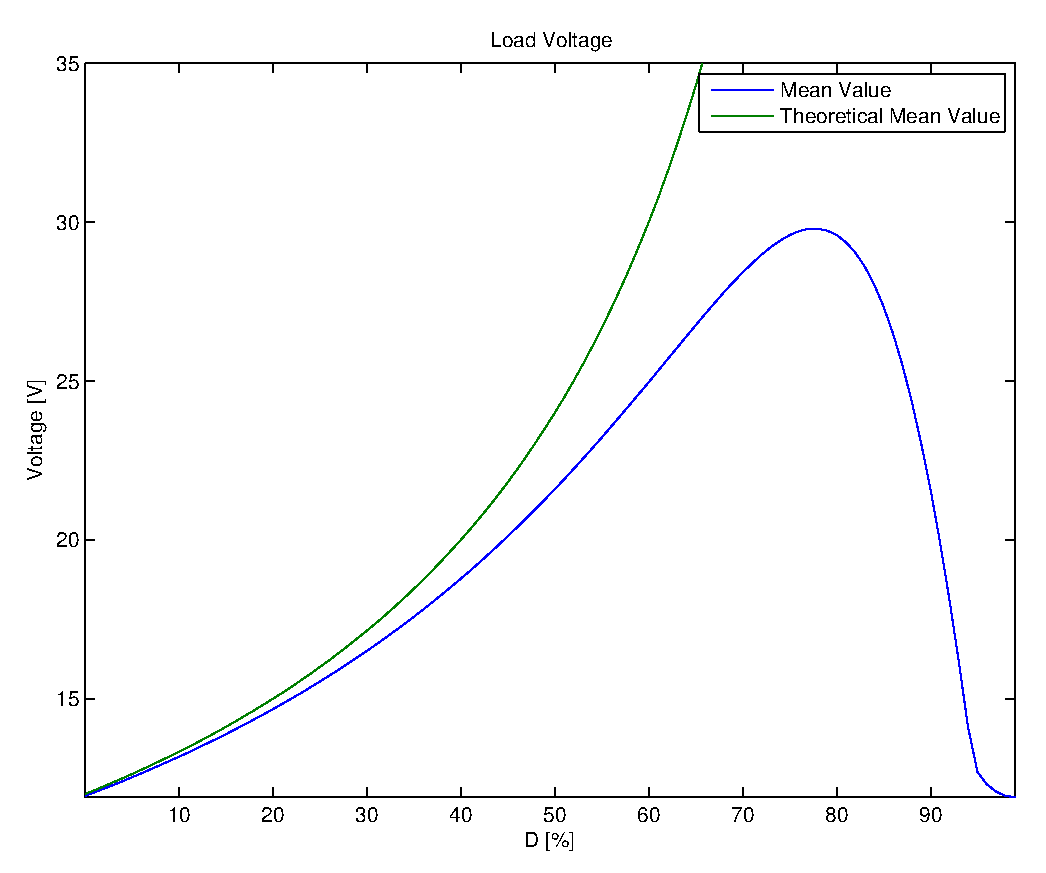
\includegraphics[width=0.7\linewidth]{matlab/boost/r_vrxd}
	\caption{Tensão média no resistor para conversor boost}
	\label{fig:bovrxd}
\end{figure}

Como podemos ver os valores obtidos são %TODO esperados teoricamente, isso se deve às imprecisões numéricas da simulação, à queda de tensão introduzida pelos diodos, ao pequeno período de amostragem, entre outros fatores.

Podemos calcular o valor da indutância limite $L_b$ para que o conversor trabalhe em modo de condução contínua utilizando a equação:
\begin{equation}
L_b = \frac{(1 - D)^2 DR}{2f_s}
\end{equation}
Para um duty-cicle $D$ = $80\%$, temos:
\begin{equation}
L_b =  3.2\mu H
\end{equation}

Ajustamos então nosso indutor para $L$ = $\frac{L_b}{2}$ = $1.6 \mu H$ e rodamos a simulação novamente, obtendo os resultados apresentados nas figuras \ref{fig:bor2}, \ref{fig:bol2}, \ref{fig:boc2}, \ref{fig:bos22}, \ref{fig:bod12}.

\begin{figure}[H]
	\centering
	\begin{subfigure}[b]{0.4\linewidth}
		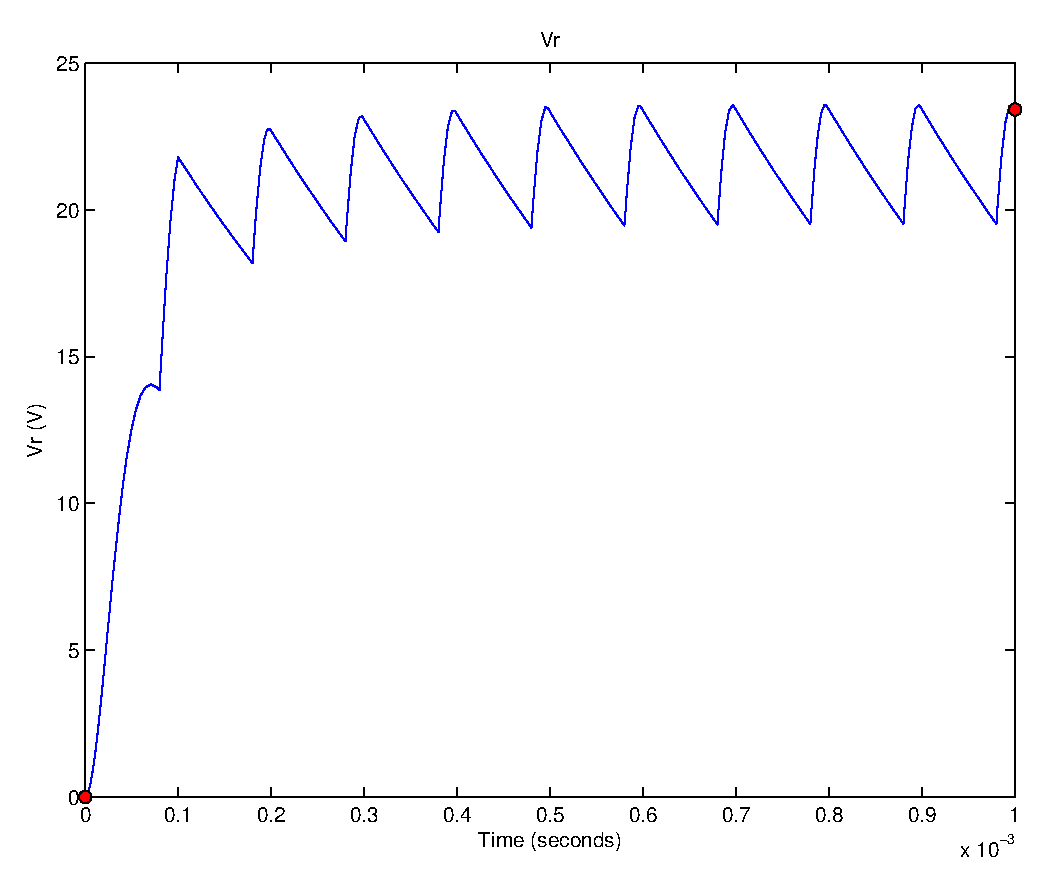
\includegraphics[width=\linewidth]{matlab/boost/b_vr2}
		\caption{Tensão no resistor}
	\end{subfigure}
	\begin{subfigure}[b]{0.4\linewidth}
		\centering
		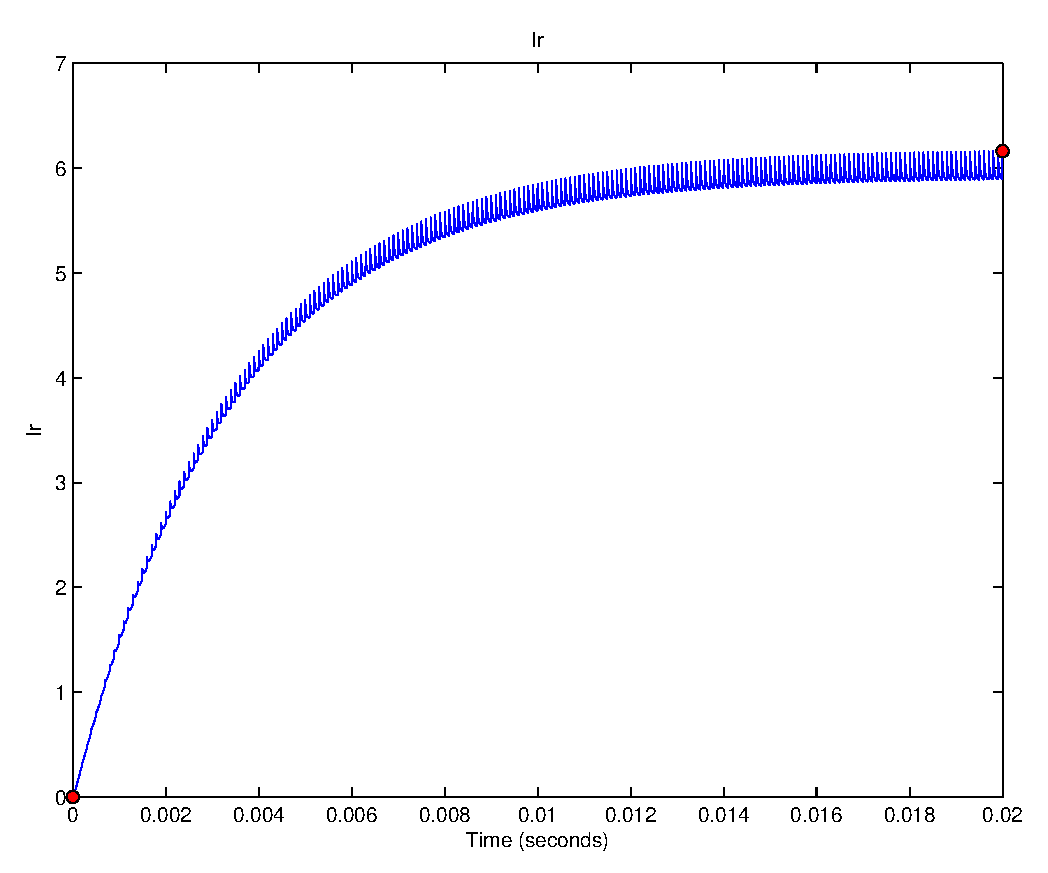
\includegraphics[width=\linewidth]{matlab/boost/b_ir2}
		\caption{Corrente no resistor}
	\end{subfigure}
	\caption{Curvas do resistor para conversor boost com indutância $\frac{L_b}{2}$}
	\label{fig:bor2}
\end{figure}
\begin{figure}[H]
	\centering
	\begin{subfigure}[b]{0.4\linewidth}
		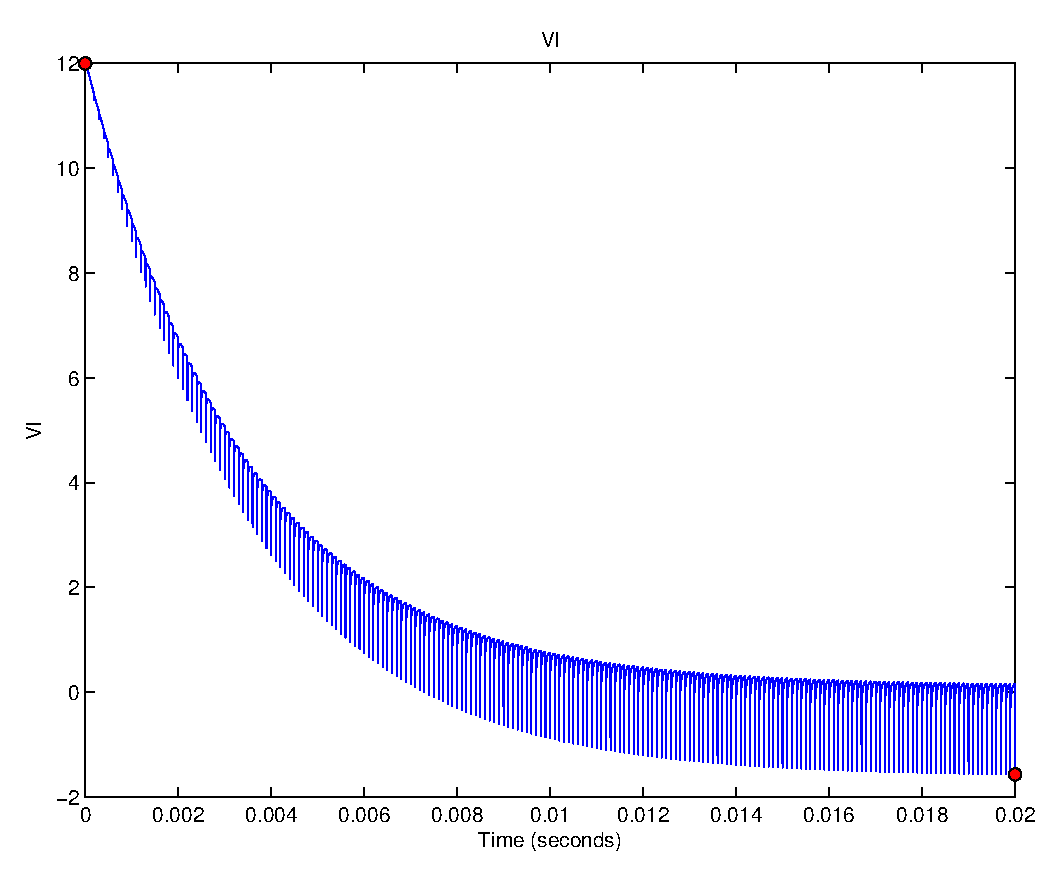
\includegraphics[width=\linewidth]{matlab/boost/b_vl2}
		\caption{Tensão no indutor}
	\end{subfigure}
	\begin{subfigure}[b]{0.4\linewidth}
		\centering
		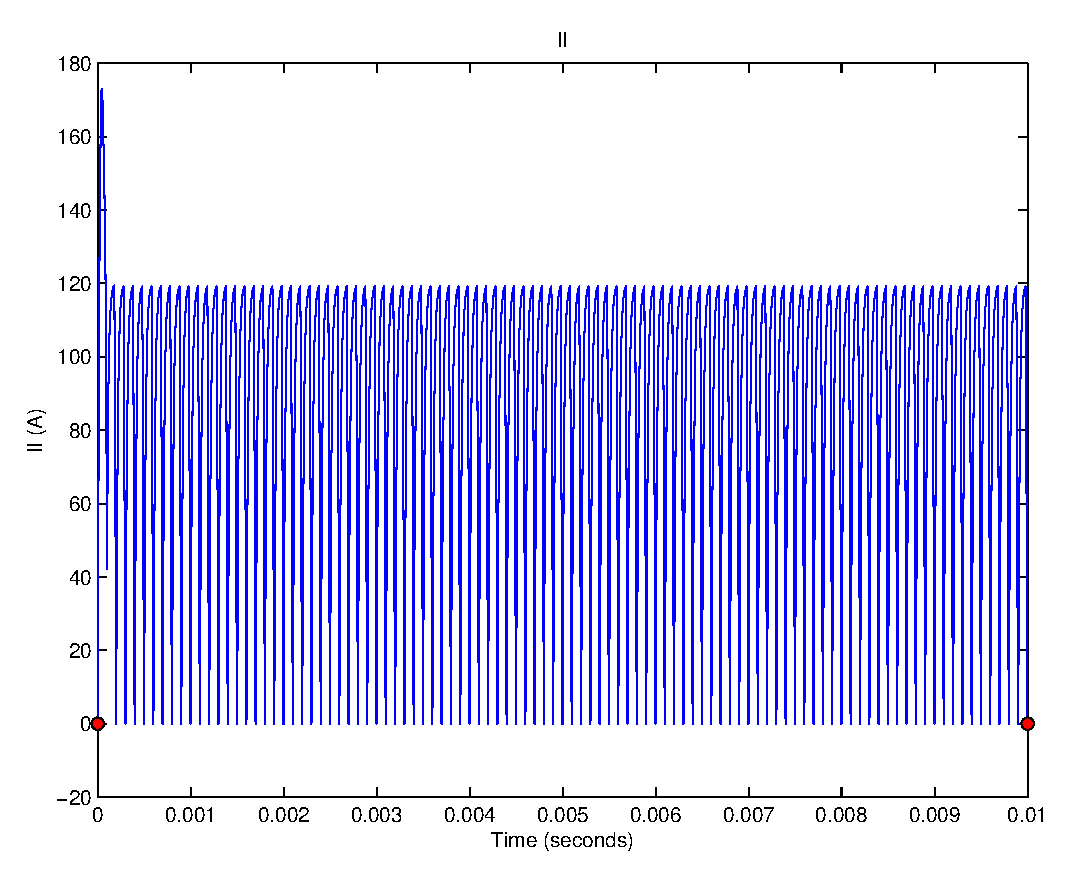
\includegraphics[width=\linewidth]{matlab/boost/b_il2}
		\caption{Corrente no indutor}
	\end{subfigure}
	\caption{Curvas do indutor para conversor boost com indutância $\frac{L_b}{2}$}
	\label{fig:bol2}
\end{figure}
\begin{figure}[H]
	\centering
	\begin{subfigure}[b]{0.4\linewidth}
		\includegraphics[width=\linewidth]{matlab/boost/b_vc2}
		\caption{Tensão no capacitor}
	\end{subfigure}
	\begin{subfigure}[b]{0.4\linewidth}
		\centering
		\includegraphics[width=\linewidth]{matlab/boost/b_ic2}
		\caption{Corrente no capacitor}
	\end{subfigure}
	\caption{Curvas do capacitor para conversor boost com indutância $\frac{L_b}{2}$}
	\label{fig:boc2}
\end{figure}
\begin{figure}[H]
	\centering
	\begin{subfigure}[b]{0.4\linewidth}
		\includegraphics[width=\linewidth]{matlab/boost/r_s2v2}
		\caption{Tensão na chave S2}
	\end{subfigure}
	\begin{subfigure}[b]{0.4\linewidth}
		\centering
		\includegraphics[width=\linewidth]{matlab/boost/r_s2i2}
		\caption{Corrente na chave S2}
	\end{subfigure}
	\caption{Curvas da chave S2 para conversor boost com indutância $\frac{L_b}{2}$}
	\label{fig:bos22}
\end{figure}
\begin{figure}[H]
	\centering
	\begin{subfigure}[b]{0.4\linewidth}
		\includegraphics[width=\linewidth]{matlab/boost/r_d1v2}
		\caption{Tensão no diodo D1}
	\end{subfigure}
	\begin{subfigure}[b]{0.4\linewidth}
		\centering
		\includegraphics[width=\linewidth]{matlab/boost/r_d1i2}
		\caption{Corrente no diodo D1}
	\end{subfigure}
	\caption{Curvas do diodo D1 para conversor boost com indutância $\frac{L_b}{2}$}
	\label{fig:bod12}
\end{figure}

%TODO ANALISAR
%\bibliography{mybib}
\end{document}

